% IT基础架构
% IT基础架构.tex

\documentclass[12pt,UTF8]{ctexbook}

% 设置纸张信息。
\usepackage[a4paper,twoside]{geometry}
\geometry{
	left=25mm,
	right=25mm,
	bottom=25.4mm,
	bindingoffset=10mm
}

% 设置字体,并解决显示难检字问题。
\xeCJKsetup{AutoFallBack=true}
\setCJKmainfont{SimSun}[BoldFont=SimHei, ItalicFont=KaiTi, FallBack=SimSun-ExtB]

% 目录 chapter 级别加点(.)。
\usepackage{titletoc}
\titlecontents{chapter}[0pt]{\vspace{3mm}\bf\addvspace{2pt}\filright}{\contentspush{\thecontentslabel\hspace{0.8em}}}{}{\titlerule*[8pt]{.}\contentspage}

% 设置 part 和 chapter 标题格式。
\ctexset{
	part/name= {第,卷},
	part/number={\arabic{part}},
	chapter/name={第,章},
	chapter/number={\arabic{chapter}}
}

% 图片相关设置。
\usepackage{graphicx}
\graphicspath{{Images/}}

% 设置署名格式。
\newenvironment{shuming}{\hfill\zihao{4}}

% 注脚每页重新编号,避免编号过大。
\usepackage[perpage]{footmisc}

\title{\heiti\zihao{0} OpenWrt}
\author{}
\date{}

\begin{document}

\maketitle
\tableofcontents

\frontmatter

\chapter{本书赞誉}

本书是一本比较难得的好书。基础架构运维工作既非常重要,又很难给出清晰描述。“运维是个筐,啥都往里装”,很多人以为基础架构运维好做,实则不然。

从数据中心水电到网络,从服务器硬件到运维自动化,十八般武艺,既要求知识深度和广度,又事无巨细。
本书以提纲挈领式的全面讲解,呈现了基础运维工作的内容,并将各个要点有机串连起来,深入浅出地贡献给读者,既可以作为基础运维工作的入门书籍,又可以作为日常运维工作的参考比照。

除了享受作者的文笔,不禁还要感谢作者为基础运维工作做出的贡献。推荐!

——刘浩,360云事业部总经理

赵兄是一个非常有经验的运维人,有着非常全面而丰富的运维知识。本书作者从数据中心、管理流程、基础服务、系统运维等多个维度来讲解对运维的理解,兼顾了流程、人和技术三个要素,更以层次化的方式自底向上剖析运维,这对一个技术运维人来说是何等的重要。喜欢运维的你,一定不要错过本书的精彩内容!

——王津银,优维科技CEO

非常高兴看到这样一本系统运维管理领域的专著出版。十多年前刚入行的时候,对系统工程师(SA)这样的职位还很陌生,之后随着支付宝系统规模的暴增,经历了一个难忘的“被成长”经历。同为支付公司运维同行,我和本书作者赵旻的成长经历类似,本书激发了我强烈的共鸣,每一个章节都能让我回想起成长的一段经历。本书绝对是来源于一线实战,又兼具理论高度。云计算时代,对系统工程师的需求和要求越来越高,希望本书的问世可以惠及更多有志于从事云计算运维的同行,传道授业解惑,让天下没有难运维的数据中心!

——智锦,杭州云霁科技CEO、资深运维从业者

当今互联网正处于快速发展的关键阶段,人工智能、大数据、VR、AR等新概念的背后,是基础架构与底层系统支持的发展和实现。没有扎实的基础架构,一切概念与创新都会变成空中楼阁。无论你是运维老鸟,还是刚刚入职的新人,这本书都有适合你的地方。

本书涵盖了数据中心规划、基础服务、系统运维等多个方面。作者以十多年的经验告诉各位读者,弯路一定是会走的,但是如何能够尽早避免,并通过行之有效的方法进行解决,才是运维管理的王道。虽然IT界一直在不停地变化,但是运维的核心精神并没有变。本书就是作者多年的运维经验的积累和沉淀,总结出一套颇具心得的IT基础架构管理法。

——李晞岩,戴尔(中国)有限公司互联网技术团队经理

本书从机房、电力、服务器等系统管理员的日常工作对象入手,既对企业IT基础架构中的各个组件进行了详细阐述,又对一线工作经验进行了提炼和升华。书中通过趣味案例的方式来传达知识,不但增加阅读乐趣,也让读者更容易理解作者要表达的重点内容,同时诱发读者思考故事中的技术点或技巧。IT基础架构是业务系统的运行基础,稳定安全是首要任务。同时,书中有关系统管理员日常工作的规范和技巧,可以帮助读者解决如何减少沟通成本、如何提高工作效率等问题。

——刘小成,热璞科技咨询交付部总监

本书内容从工作实践出发,是作者多年积累的运维经验和感悟汇聚之作。更加难能可贵的是,作者从通俗易懂的角度,图文并茂地讲述每一个主题,从而让大家理解系统运维管理之道。我认为,不同技术阶段的运维人员都能从书中吸取有益的内容。

本书也可作为运维管理建设中的指导性书籍,或许你能从书中发现自身企业运维管理的痛点,并进行有针对性的改善。感谢赵旻能给运维从业者带来这么好的分享。

——齐代英,贝壳金控资深运维工程师

\chapter{序}

和赵旻认识很长时间了,赵兄技术专业,经验丰富,逻辑性强,善于总结。当前,人工智能、物联网、云计算等新兴技术层出不穷,同时也带来数据爆炸性的增长。为了应对数据爆炸性的增长,保护这些信息的安全,基础设施的可靠、稳定尤为重要。离开了稳固的基础设施,就没有我们的现代化社会。基础设施涉及从硬件到软件、从技术到流程各个层面的知识,内容非常广泛,如何管理好基础设施,知识点非常多。赵旻的这本书很好地、系统化地总结了基础架构知识,相信能够帮助工作中涉及基础架构的工程师,快速成为基础架构领域的运维专家。

本书有三个特点。

第一,道术结合。

每部分内容,从原理开始,然后介绍实践。因为作者从事基础架构多年,经验丰富,在工作中不断地总结升华,所以原理总结得深刻简明,切中要害。实践方面不但都是干货,而且在组织方面充满逻辑性。阅读本书的时候,读者会觉得非常有条理感,很容易接入自己的知识体系。

第二,广泛的维度。

本书涉及广泛的基础架构知识,既包括空调水电、硬件、网络、软件方面的技术,又涉及流程、管理等方面的知识,并分享了工程师自我提升的经验。每一部分都不是简单地提及,而是深入论述,许多部分还附有案例。

第三,充满诚意,充满干货。

本书有13个运维故事,每个故事都是作者精心选择或设计的,可见作者为了表述清楚自己的观点,下了很多工夫。许多知识点,作者都进行了详细的讨论。例如关于闰秒这一节,作者讨论了“闰秒是什么,闰秒的危害,前辈们是怎么解决闰秒的,晦涩难懂的术语,怎么解决闰秒问题”几个话题,通过这一节的阅读,读者不仅可以对闰秒有深刻认识,而且还知道了闰秒相关的历史。再如关于服务器硬件的测试,作者分为“测试前的准备工作,部署系统测试,产品功能性测试,能耗测试,CPU性能测试,内存性能测试,磁盘性能测试,网络性能测试,测试后的收尾工作”几个主题,通过这一节的阅读,读者可以对服务器测试的知识点了解得清清楚楚。类似的地方,书中还有很多,等待着读者来体会发现。

本书是强强联合的出品,本书的作者赵旻是业内著名基础架构专家,本书的编辑高婧雅是知名编辑。高编辑我非常熟悉,工作方式用一个词总结就是“认真”,在选题审稿方面会和作者死磕,正是因为高编辑的认真,高编辑参与的书基本都是精品,本书也不例外。

肖力 云技术社区创始人

\chapter{前言}

2015年,国务院政府工作报告中提出制定“互联网+”的行动计划。在这个大背景时代的推动下,越来越多的传统行业面临着与云计算、大数据等热门技术相结合的发展趋势。在漫长的转型过程中,传统企业的IT部门面临着基础架构变革的严峻考验,运维团队不可避免地遇到了很多棘手的难题。例如,管理模式如何由集中式向分布式转型,小型机到x86的演变,海量运维模式的挑战,以及知识结构与运维思路的转变,等等。这些都是目前传统行业IT部门领导者所面临的主要问题。

随着电商的流行,也有很多非IT领域的成功企业正在酝酿着自己的O2O市场,希望借助互联网完成第二次创业。他们遇到的最大问题就是——对互联网的认知完全是一片空白。要实现从无到有的原始积累,会有很多挑战在等着他们。

\section{为什么要写这本书}

基于上述这些问题,我们策划了这套IT基础架构丛书。作为这个系列的第一部作品,我个人的压力还是蛮大的。当机械工业出版社华章公司的高婧雅编辑和我约稿时,自己竟然一时有些不知所措。算起来,我从事系统运维的工作已满十个秋冬。说来惭愧,我觉得自己并没有什么拿得出手的成绩。不论是实践还是基础,市面上这方面的书已经非常多了。那么,以什么作为出发点是合适的呢?最终,我还是从《运维前线》\footnote{已由机械工业出版社出版,书号978-7-111-55697-8。—编者注}这本书中获得了启发。2017年3月,由云技术社区创始人肖力发起并策划的《运维前线》成功出版,让我感受到了同行们乐于分享的热情,同时也看到了广大读者对实用、落地的技术方案的渴求与肯定。于是,我产生了一个新的想法:在《运维前线》主打实用的基础之上,围绕着我所擅长的系统运维方向,写一部《运维前线》的“系统版”。

\section{本书特色}

不管怎么说,技术是一个很枯燥的东西。我自己在学习的过程中也深有体会。拗口的描述、复杂的逻辑是很多技术文档的通病。也许这样的表达形式是严谨的,但它并不“亲民”。我认为,一本好书不但要有深度,更要带领读者一同到达才行。这个深度就像西游记中的水帘洞,如果只有你自己进去了,却把读者晾在一边,那真是太糟糕了。如果一本书洋洋洒洒几十万字,读者看完后没有任何收获,那我宁愿不去写它。因此,打比方和举例子是我在全书中用得最多的写作手法。通俗易懂,是我在技术分享时所秉持的一贯态度。我希望消除掉一切阻碍的门槛,让每一位读者朋友都能够从本书中获得些许的帮助。

选择撰写本书是有着特别的意义的。既然是实践,我们首先要保证技术的实用性。但从定位上讲,它又不同于以往的实践类书籍。书中讲述的所有内容都是笔者正在或者曾经使用过的,并将一些经验和观点融在其中。写这本书,也算是对我多年工作经验的一种总结,了却自己的一桩心愿吧。

\section{读者对象}

说到这本书的定位,我想它对绝大多数从事系统运维的工作者都是有益的。本书需要一点点Linux和网络的基础知识作为铺垫,除此之外再无其他要求。对于工作3~5年的朋友们,我知道你们已经厌倦了基本的系统管理,但你们也许有点儿迷茫,不知道下一步该如何进阶。对于那些传统行业面临IT基础架构转型的系统运维团队,你们可能在系统管理方面经验丰富,但是对大规模、分布式x86平台的系统运维却感到陌生。还有那些刚刚到创业公司的“中生代”技术人,你们可能在工作中会遇到更多新的挑战。我想,选择这本书对你们来说是再适合不过的了。当然,如果你早已是这方面的行家里手,也不妨来读读本书。我的一些经验也许能帮到你,我的一些经历也许能让你感同身受,我的一些观点也许能让你会心一笑,只当是我与你之间的一次未曾谋面的技术交流好了。

\section{如何阅读本书}

本书从内容上大致分为六大部分,共计16章内容。

第一部分

(第1章),笔者对心中的IT基础架构标准、本书的写作初衷和特点等做了阐述。

第二部分是数据中心篇

(第2~5章)。这是一个综合了数据中心、网络、系统等众多技术领域的主题。我作为一个经历过创业公司的老员工,对此深有体会。从无到有,我亲手规划、建设了多个同城的数据中心,后续又和两位牛人学习了很多相关的知识。该篇也许真的非常跨界,我想在所有讲解系统技术的书籍里,难有雷同之作。作为一名真正的SE,只懂操作系统是不合格的。所以,我认为这个跨界还是值得的。

第三部分是管理流程篇

(第6章)。这是一个特殊的篇章,因为它特殊到只有一章。如果能够进一步展开,这个主题其实完全可以独立成书。管理流程是基础架构中最为重要的核心组件。我想没有人会反驳这个观点,除非他所运维的节点数量还不够多。

第四部分是基础服务篇

(第7~11章)。本篇内容基于多机房和海量节点,介绍了如何去构建DNS、NTP、文件共享、配置管理等一整套服务的方法。

第五部分是系统运维篇

(第12~15章)。这部分内容主要和日常运维管理的工作相关。例如,硬件故障处理与维修、安全、性能校准、Shell程序等。如果要做推荐,我会更倾向于数字证书那一章。因为那是我刚入行时的专业方向,和数字证书打了这么多年的交道,写这一篇时也算是一种情怀吧。

第六部分

(第16章),这部分介绍系统运维工程师应该具备的素养,以及如何提升自己等内容。

此外,这本书中还有13个有趣的运维小故事。它们很像登山时的休息点,如果你读累了,可以在这里歇歇脚,喘口气。其实,故事里面也蕴藏着很多收获呢。

不过,这还不是本书全部的内容。既然我受到了《运维前线》的启发,为了表示敬意,我也继承了《运维前线》一书的设计形式。最后一章,藏着一个有趣的彩蛋,等待着读者朋友们去发现。好了,我想我说得已经够多的了,我们在书中相见吧。

\section{勘误和支持}

由于笔者的水平有限,编写时间仓促,书中难免会出现一些错误或者不准确的地方,恳请读者批评指正。如有任何反馈与想法,请你发送电子邮件到itarch@qq.com。真诚地期待能够得到你的反馈,在技术之路上互勉共进。

\section{致谢}

在写作这本书时,我得到了很多朋友的帮助。例如我的同事——张望和徐铁军两位大牛。张望是网络方面的专家,铁军则有着多年的IDC管理经验。撰写数据中心篇章时,关于一些技术问题的求证,两位给予了我很多的支持与帮助。能和你们在一起工作真好,谢谢两位。

感谢云技术社区的北极熊,熊总在各大社区中不遗余力地帮忙推广本书,做了很多无私的工作。感谢我的那些新老朋友们,在我成书之时,他们帮我撰写书评,给了我很多的鼓励与支持。谢谢你们的帮助与肯定。
此外,在这里我还要特别感谢两位老师。一位是云技术社区的肖力,另一位是机械工业出版社华章公司的高婧雅老师。两位老师是指引我走上写作道路的领航人,虽然都只有一面之缘,但他们却给我提供了很多的帮助和支持。2015年,我加入了力哥发起的《运维前线》的写作团队。也正是通过这次写作得到了婧雅编辑的肯定,进而才有了这部书稿的成文。力哥在百忙之中亲自为我作序,婧雅为我的写作提供了很多有价值的指导意见。可以说,没有两位就没有这部书的出版。谢谢所有支持我、关心我、帮助我的朋友们,感激之情溢于言表,谢谢大家!

谨以此书献给广大热爱技术的朋友们!

赵旻

\mainmatter

\chapter{混沌初开}

混沌未分天地乱,茫茫渺渺无人见。

自从盘古破鸿蒙,开辟从兹清浊辨。

在这里,首先要感谢你能选择这本书。我已经很多年没有动过笔了。自打高考结束之后,我就很少再有机会爬格子了。这一切还是托了肖力兄的福。通过《运维前线》这部书,我结识了很多同行好友。也承蒙力哥和机械工业出版社华章分社的高婧雅编辑的鼓励与错爱,再一次燃起了我的写作热情。

\section{我眼中的基础架构}

相传战国时期,魏国的国君魏文侯外出巡游,在路上遇到了一个反穿裘皮大衣的人。魏文侯觉得很奇怪,向那人问道:“你为何要将衣服的毛穿在里头,却把皮板露在外面呢?”那人回答说:“这件裘皮大衣很贵,我怕损伤了毛,所以才这样穿的。”魏文侯大笑:“难道你不知道,要是这皮板磨破了,毛也就保不住了吗?”

古人云:“兵马未动,粮草先行。”没有必要质疑基础架构的重要性。2015年至2017年可以称得上是互联网界的“三年灾害时期”。重大事故频发,很多知名企业先后“中枪”,在业内引发了很大反响。其中大多数故障与基础架构有关,从这些事件上折射出了很多问题——我们对基础架构的重视和投入是不足的。

其实“平日不烧香”倒也没什么关系,只要事后你能平心静气地承受所有的损失,不要哭天抢地、痛心疾首就好。这和买保险是一样的,投100万元还是100元,完全由你决定。但有一点我能肯定,你觉得你的基础架构值多少钱,你就会去投入多少。

做基础架构,我认为有三点非常重要——可靠、简单和高效。

1.可靠

可靠是毫无疑问的。如果底层不扎实,上面再花哨也没有用。不少企业在建设初期,为了抢占市场、追赶进度,相对于产品开发,基础设施的建设往往滞后得非常厉害。我在本书的第6章,特别强调了基础架构中的两大基石——CMDB和Workflow的重要性。试想如果没有CMDB,你的信息从哪里来?没有规范的Workflow,如何确保信息的准确性?把精力放在基础架构的建设上,要比盲目求高、求快有意义得多。

可靠性不仅仅体现在软件架构上,基础设施的可靠性同样重要。基础设施在可靠性上栽跟头的主要原因就是钱。财务、采购和技术部门经常在成本价格上发生冲突。一边要节约成本,一边要提升服务等级,每个部门都在追求自己的价值体现。部门的话语权就决定了你是否会掉进低价陷阱之中。廉价、免费是世界上最昂贵的商品。看似便宜的东西,买回来就会大呼上当。不是品质打折扣,就是后期产生无尽的费用增项。这种“抠小钱、舍大钱”的做法是非常不值的。

2.简单

简单是支撑规模增长、消除扩容瓶颈的基础要件。架构的复杂度和今后发生事故的严重程度是成正比的。底层架构的逻辑越复杂,出问题以后牵扯的东西就越多。真是因果循环、报应不爽啊。

不同的体量,架构的实现模式会有不同。因而随着规模的增长,你的架构会不自觉地增加复杂度。这是不可避免的,所以架构师要不断地为新架构减负和解耦。在削减赘肉的过程中,我们要消灭基础架构身上的三座大山。

第一,要消灭异构形式。

不论是通信协议、接口规范抑或实现方式,最忌讳的事情就是大家各玩儿各的。你做一个标准,我做一个标准,每接入一个新的子系统,就要产生很多兼容性问题,最后还不是要花大力气去融合么?

第二,要消灭重复组件。

底层功能的实现在业界大多有成熟的解决方案,应当尽可能地去复用或者在此基础上进行改进,而不是重复造轮子。研发精力要更多地放在业务场景的适用性上。

第三,要消灭紧耦合关系。

解耦工作要从不同的角度入手,子系统和模块的紧耦合因素是不同的。

实现系统间的解耦要让架构扁平化,消灭冗余的层级。垂直层面上的内容越多,就越容易出问题。如果执行一项任务要历经十个系统。一旦任务失败,这十个系统都脱不了干系。另外,在需求迭代的过程中,每增加一个需求项,不论你所负责的系统是否需要修改,在任务没有明确之前,这十个系统的开发人员都得参与讨论。不断地开会,不断地沟通,你想这些成本代价得有多大?

实现模块间的解耦要明确职权界限。调度模块只负责调度,部署模块只负责部署。假使调度模块在调度过程中发现,环境的初始化工作没做好(例如缺少某个配置文件),那么它应当给部署模块返回错误消息,而不能让调度模块去做拉取文件的动作。如果开发任务指派了多个人去完成,则这种问题就很容易发生。等于两个模块里面都有部署的动作,它们之间的界限就模糊了,从而出现多头管理的问题。

解耦的核心是拆除过度的依赖关系,让暴露给外部的细节最小化,形成“高内聚、低耦合”的最优状态。

3.高效

团队工作的特点是人多省力、人少省心。当一件工作从一个人干变成十个人干时,你会发现信息来源的权威性、信息同步的实时性和操作指导的规范性有多重要。当运维团队增长到一定规模的时候,效率反而会有所下降。因为工作被进一步拆分了,在缓解压力的同时,相互之间的衔接环节却增多了,沟通成本以及利益冲突的负效应也会在这个时期显著放大。

影响效率的主要因素来自于CMDB和Workflow模型的成熟度。具体细节我们就不在这里过多讨论了。总而言之,基础架构做不好,整个团队的管理是一片混乱,执行效率低下,成员怨声载道。俗话讲:磨刀不误砍柴工。把精力多放在基础架构的建设上是绝对不会吃亏的。

\section{写一本怎样的书}

在策划这部书的时候,我受到了《运维前线》的很多启发。2015年,我有幸加入了首部《运维前线》的写作团队。从《运维前线》的创作到出版,不仅让我感受到了同行们乐于分享的热情,同时也看到了广大读者对于实用、落地的技术方案的渴求与肯定。于是我有了一个新的想法:能否在《运维前线》主打实用的基础之上,再让它更加系统、丰富一些呢?

选择撰写这部《IT基础架构:系统运维实践》是有着特别的意义的。在定位上,它不同于以往的实践类书籍。当然,既然是“系统运维实践”,我们首先要保证技术的实用性,必须回归到具体操作的实例讲解中来。什么是实践?我想绝对不是在虚拟机上呈现一个实验结果那么简单。如果只是这样,你完全可以在互联网上找到很多类似的文档,这不是我想要的。真正的实践,一定要是你亲身用过的东西,有宝贵的经验之谈在里面。我们从来就不缺少安装文档,读者需要的是——站在架构层面上的技术应用指南。这,才是我写作的初衷。

当然,基础架构这个题目很大,绝非我一人之力所能承担,所以我并非一个人在战斗。我希望能沿用《运维前线》的众筹创作模式,汇聚业内众多专家,总结他们多年的工作经验,从而形成一套通用的解决方案模型,使之可以应用于大部分的场景。也就是说,作为抛砖引玉之作,本书只是“IT基础架构”系列丛书的第一部。我们正在邀请更多的作者加入到这个项目当中。我相信这是善举,愿这套“IT基础架构”丛书能成为真正落地的解决方案。就像马云所说的,让技术为大众去服务,而不是成为牟取暴利和树立壁垒的手段。

\subsection{英文书的伤痛}

有很多人曾经都问过我,学习Linux应该看些什么书。我的建议是,最好先去读Redhat OD(官方文档)。它的权威性是不言而喻的。阅读OD时,你的心里是踏实的。尤其是到达一定技术深度的时候,知识来源的可靠性非常重要。不过很多朋友表示看OD有难度,主要是英文不过关,这一点我也是感同身受。

翻译专业文档的确是一件极其辛苦的工作,要做到“信、达、雅”谈何容易?一方面我们对于专业词汇的理解不到位。另一方面,外国人的某些表达方式与我们不同。明明很简单的道理,偏要花几大段英文来解释。而拆解成两三个短句能说清楚的事情,却非得用一个超长从句来表达,还有各种which与it的不明指代。这让我深感英文依旧是我们技术进步的最大障碍。

在讲解一些来源于英文文献的内容时,为了弄清楚各种专业词汇,我翻阅了大量的资料。例如,在时间同步这一章中,像slew、smear这类单词,即便你知道它们的原意,也未必就能很好地将其代入实际语境当中。而且就算翻译到位了,读者对专业词汇的理解也是吃力的。在充分理解原句含义的同时,再用浅显易懂的语言描述出来,我在这方面也着实是费了一番工夫的。

\subsection{有话直说——这就是我的忍道}

我中学时代的一位语文老师在给我们讲写作时,曾举过一个特别生动的例子。当时中学作文的字数限制是八百字。她说,文章开篇一定要平铺直叙,快速切入主题,字数不要超过一百。写作文就像打仗,这八百个字就是打仗时你率领的士兵。有些同学写作文开篇太啰唆,一冲锋都死伤一百多个兵了,结果还不知道你要说的是啥呢。

事实上,我自己也特别痛恨这种说话兜圈子的方式。如果一部书洋洋洒洒几十万字,读者看完后没有任何收获,那我宁愿不去写它。我不能变成自己所讨厌的那种人。现在大家提倡讲干货,就是因为有些技术分享已经开始变味儿了。举几个例子,我想大家一定都有同感。

(1)白皮书式的分享

白皮书式的分享就像是一个销售在推销,全程围绕着一张架构图,依次介绍里面每一个模块的名字和作用,最后展示一张效果图。分享结束后,听众发现自己和这个产品完全没有任何交集。其实,大家并不关心这些模块叫什么,做什么用。我们真正感兴趣的是,整个系统的工作流程是怎样实现的,模块之间是如何协同工作的,在实现过程中遇到了什么问题,又是如何解决的,这套系统适用于哪些场景,在什么时候会遇到瓶颈,这个模式我们能复用么?然而,这些问题都没有给出答案。

(2)炫富型的分享

我觉得这种分享根本就是来“拉仇恨”的。巴拉巴拉讲了一个特别牛的产品,最后话锋一转,说这是我们团队自主研发的。言外之意就是——你们用不了!

(3)表演型的分享

技术分享的目的是让大家获益,而不是用来突显你有多高明。有些分享特别热衷于过度包装,非要把简单的东西往复杂里说,刻意地堆砌各种术语以及模型公式,却又不做任何解释。这种做法完全不顾群众的接受能力,似乎一开始就没打算让你弄明白。

从上述这几个问题来看,我认为分享人的内心并不是真正开放的。写书也是一样的道理,读者并不是傻子,你自己内心的拧巴与纠结,大家看得很清楚。

如果非要下一个定义,我认为《IT基础架构:系统运维实践》是一部抽象化的实践类手册。这里面既有模型和方法,也有案例和步骤。作为抽象化的架构设计,我会交代清楚它的原理、构想以及我们为什么要这样做。作为具体的事例,我要确保它是切实可行的。读者完全可以复用到大多数场景中去,因为它们都是笔者曾经或者正在使用的技术方案。

一部书有没有价值,并不在于技术的深浅,而在于作者的诚意——有没有分享干货的意愿。我愿意尽我所能去帮助任何有需要的朋友,相信这是一部脚踏实地、有一说一的书。有话直说,这就是我的忍道。

\subsection{当行家说人话}

我入行是从信息安全做起的,那时我在政府行业中做了很多国家级项目。其中某部委的一位领导,给我留下了很深的印象。有一次,我们的项目经理提交了一份文档,被她给打回来了。她让项目经理当场高声朗读这份文档。这一读不要紧,项目经理自己也觉出来了,文中语病甚多。这位领导斥责道:如果你写的文档连你自己都读不明白,怎么好意思拿给别人去看?

这件事对我的影响很深。程序员写完代码要自测,作者写完文章要自读。而且一定要念出声儿来,这一点很重要。朗读能够从心态上清空自我意识,从一个读者的角度去读自己的文章,你是不是真的能读懂你所说的话呢?

当行家、说人话,是我这次秉承的写作态度。为了避免出现“看不懂、读不通、想不明、理不清”的情况,这一部长达30万字的书,我至少写了50万字的内容。即便是这样的一个开篇,我反反复复地也删改了很多次。有时我真的很痛苦,利用通宵及周末加班写出的大段文字,最后很多都被自己删掉了。忙了几天,却发现Word的字数统计几乎没有变化。我不是职业作家,交稿的时间也很仓促,要说没有压力是骗人的。其实在临近截稿前,我感觉自己就像是一个高考结束铃响时还在奋笔疾书的考生,很想能有更多的时间来细细打磨全书。因为我希望这部书的内容能更加完善,有些呆板干涩的地方,也许还可以将它润色得更好一些。此外,我也担心因为自己的一时疏忽或者知识上的空白,而给本书留下一些错误。读者朋友们,如果你在阅读的过程中发现了任何问题或疑问,欢迎你提出批评和建议,我将在下一版中进行改进。如有任何反馈与想法,请发送电子邮件到itarch@qq.com。再次向你表示感谢。

\section{本书声明}

在拟定本书目录之时,高婧雅编辑曾经给我提过一些建议,她希望本书能够有一些实际案例的讲解。我原本就有培训的工作经验,而举例子和打比方又是我喜欢的讲述风格,所以列举案例对我来说不是问题。但我又有点儿为难,案例中难免会有些反面典型。但做运维的人,谁没开过故障分析会?谁没犯过错误?案例分析不是要针对谁,而是为了达到总结经验、吸取教训、警醒后人的目的。在此我郑重声明,本书列举案例所涉及的公司和人名均为虚构,一切只为说明问题,请勿对号入座哦。你要是较真儿,那我就只能说清者自清了。还是那句老话,本书故事纯属虚构,如有雷同,实属巧合。

在撰写本书时,笔者参考了很多非常有价值的资料。有些源于Red Hat的官方文档或软件的用户手册,一些名词解释和介绍性的内容来自互联网,还有一部分摘录自笔者已经发表在《运维前线》上的文章。

除此之外,在撰写本书的第8、10和14章时,笔者还参考并借鉴了如下书籍中的部分内容。在此,我对这些书籍的作者们深表敬意。

[1] Cricket Liu,Paul Albitz.DNS and BIND[M].5版.纽约:O扲eilly Media,2009.

[2] 克鲁姆,等.精通Puppet配置管理工具[M].李超,译.2版.北京:人民邮电出版社,2014.

[3] 李松涛,魏巍,甘捷.Ansible权威指南[M].北京:机械工业出版社,2016.

[4] Joseph Hall.精通SaltStack[M].姚炫伟,译.北京:电子工业出版社,2016.

[5] 莫尔勒.深入Linux内核架构[M].郭旭,译.北京:人民邮电出版社,2016.

[6] Redhat,Inc.RedHat.System Monitoring and Performance Tuning:RH442[EB/OL].https://www.red-hat.com/en/services/training/rh442-red-hat-enterprise-performance-tuning.

\chapter{如何选择优质的数据中心}

信息化是当今世界经济和社会发展的大趋势。谁能够掌握更多、更准确、更及时的信息数据,谁就能在这个时代的发展大潮中占据主动与先机。毫不夸张地讲,对信息数据的有效掌控,将成为企业的核心竞争力。

对于小微企业和个人创业者而言,租用公有云是个不错的选择。尤其是那些非IT企业,租用公有云可以免除日常维护的烦恼。然而,随着企业规模的不断壮大与数据量的急剧增长,公有云的弊端就会逐步显露出来。

第一,业务增长导致存储和计算节点的需求激增,成本价格会成为扩容的最大障碍。

第二,公有云数据托管的安全问题一直备受争议。作为命脉的核心数据,又岂能轻易地托付于人?

因此,公有云的应用是有很大局限性的。

在“互联网+”这个大趋势之下,IT基础架构也面临着变革的考验,以x86平台为代表的大规模集群、分布式的架构必将成为主流。因此,建设一个高可靠、大容量的数据中心的必要性就不言而喻了。

\section{概述}

数据中心的建设有两种方式。

第一种是采取机房自建的方式,它的优势在于满足定制化需求和后期的成本控制。但是,对于大多数企业来说,机房自建是一个相当复杂而庞大的工程。光国家标准规范就有上百部之多,需要很多专业人员参与,而且初期投资巨大,没有一定的规模,自建是得不偿失的。

还有另外一种切实可行的方式:选择一家优质可靠的数据中心,把自己的设备托管给服务商,这种方案是大多数企业的首选。不过,我们在数据中心的选择上可能没有做足功课,因为选择了一家不靠谱的运营服务商,导致业务中断、数据丢失的案例也不止一两起。

对于数据中心存在认识上的误区,我想这是问题的主要原因。大家可能总是觉得,机房工作不就是上架、布线嘛,很简单啊。那不过是日常工作而已。数据中心的建设和维护其实是一门涉猎非常广泛的学问,涵盖了地理学、建筑学、工程预算、管理学等诸多内容。想成为这个行业的佼佼者,只有技术是不够的,至少要在以下三个方面有所成就。

·专业知识——专业知识过硬是最基本的要求。

·行业情报——如果一个人深谙行业内的来龙去脉,而且总是能够第一时间了解到最新的相关消息,那么他的价值远非单纯的技术专家可比。

·人脉关系——关系的重要性自不必解释。深厚的人脉关系往往能趟平很多看似困难重重的坎儿。

\subsubsection{运维故事1:水火相容}

Forever和Never是两家互为竞争对手的公司。Forever公司IT部的架构师老Z跳槽去了Never,正赶上Never正在筹划新的三地多机房数据中心,为了一显身手,老Z把Forever已经完全成熟的网络架构方案直接照搬给了自己的老板。这个架构的骨干网涉及一个问题:需要两家大型电信供应商Conflagration(火灾)和Flood(洪水)之间的链路完成互通。光看名字,就能明白这两家是世仇,可见想要实现竞争对手之间的链路互通谈何容易?老板甚至都有点儿怀疑当初聘请老Z这件事是不是有点儿不太靠谱儿。老Z自己觉得很委屈,以前在Forever的时候明明就是很容易实现的啊?他百思不得其解,于是只能给原来的老同事——Forever公司负责数据中心的经理老D打了通电话。

在听完老D洋洋得意的一番解释之后,他这才明白其中的缘由。原来老D可不只是个搞技术的,人家在IDC行业摸爬滚打了20多年,除了技术水平高,更重要的是对这里的市场行情和人脉关系门儿清。Conflagration的老总和老D早先是老同学,俩人私人关系一直不错,而Flood的高层和老D是多年的好哥们儿。所以,这趟活儿人家是托了人情的,能顺利促成也无非都是冲着老D的面子,而非像老Z那种想当然。当然,按照老D的话讲,他为了这个项目,也是把这些年积攒的人情面子一次性地全给用光了,要不是老板再三保证能给自己升职加薪,他才不会这般自讨苦吃呢。

既然数据中心如此重要,那么如何选择一家优质的数据中心呢?大家也许会说,那还不简单,找一家口碑好的不就行了?要不,就招一个数据中心专家来解决。我们是做系统运维的,这和我们又有什么关系呢?

其实,在开始写作之前,我还和高婧雅编辑就这个问题多次探讨过。系统运维扯上数据中心会不会偏离了主题呢?会不会让读者觉得枯燥呢?但是当我真正地完成了这章内容的写作时,我已经对此有了足够的信心。

从数据中心的角度讲,藤上的甜葡萄早就被人摘光了。好的数据中心有可能因为用户众多,在容量上无法满足你的需求。另外,数据中心也不是简单看看评级和口碑就能够下结论的,同级别的数据中心之间也会有很多差异。

从人的角度讲,请一位资深专家在成本预算上是比较高的,大多数情况下,这项工作可能是以兼职的形式出现的。而数据中心又是一门广泛而复杂的学问,真要去系统地学习,恐怕短时间内难以有所作为。

实话实说,我并不是数据中心方面的专家,连专业都谈不上,所以我不打算把文章写得过于理论化。相反,我会用一些浅显易懂、轻松愉快的方式来讲述。

\section{空间环境评估}

从本质上讲,数据中心也是一栋建筑物。就和我们买房一样,在地理位置和房屋结构的挑选上,也需要仔细斟酌。数据中心的选址工作非常重要,地理位置决定了数据中心的安全性以及工作的便利性,而牢固的建筑结构、合理的空间布局同样非常关键。

2015年8月12日,天津港发生了特大爆炸事件。爆炸同时引发了周边地区多起火灾及二次爆炸事故,方圆数公里都有强烈震感。而位于事发地点附近的某个大型数据中心在此次事故中受到了严重冲击。由此可见,数据中心的选址工作是多么重要。

我们再来看一个场景。某客户近日需要紧急上架200台服务器。但不巧的是,当日天气突变,运输的货车刚刚到达,转眼间就下起了倾盆大雨。数据中心既没有可以避雨的场地,室内也没有充足的空间来临时放置设备,大家只好在心里默默祈祷,希望这场大雨能早一点儿停下来。从这个案例中可以看出场地条件对工作开展的限制与影响。

\subsection{地质环境}

我们在选择数据中心的时候,尤其是用于灾备的异地机房,一定要做好充分的考察工作,确认数据中心所处的地理位置是安全的。

由于我国位于亚欧、太平洋、印度洋三大板块的交界处,这样的地理位置使得构造断裂活动强烈,常年均有不同程度的地质灾害发生。南部地区降水多,泥石流、洪涝灾害比较严重。尤其是西南方向,青藏高原、云贵高原以及四川盆地是地震、山体滑坡、泥石流的多发地带,四川汶川和青海玉树近年来都发生过特大地震灾害。北方的华北地区也属于地震多发带。此外,华北、西北地区还会因为地表水不足和开采过度等原因出现沉降带。而东南沿海方向,主要是受到塌陷和海啸的侵袭。

简而言之,我们选址的主要目的就是为了躲避天灾和人祸。我们要做到五个远离、三个临近以及一个确保。

(1)五个远离

五个远离是指数据中心应远离水、土、火、污、磁这五大区域。

·洪涝区域,水库堤坝下游,沿海航道,江河湖泊。

·山地滑坡、泥石流地带,火山、地震、地质断裂带,低洼、沉降带。

·化工厂、加油站、面粉厂等地。

·核电站或者重污染源(包括噪声污染、化学污染、粉尘污染等)。

·发电站、变电站、铁路、机场等地会产生较强的电磁干扰,对设备的正常通信和信号接收造成影响。

(2)三个临近

三个临近是指临近交通、运输和生活区。

·临近市政主干道,便于设备运输。应当具有两条以上可直连主干道的道路,确保不会发生运输线中断事件。

·临近公共交通站,为来往提供交通便利。

·临近城市及生活商业区,方便工作人员在附近就餐及安排住宿,为驻场值守工作提供便利。

(3)一个确保

一个确保是说,要确保该地区有良好的移动信号,保证联络通畅。

更多的细节,我们可以参考《计算机场地通用规范》(GB/T2887——2011)。不过,在这里提示大家注意,千万不要走极端。比如加油站,它像一个巨大的储油罐,起火爆炸后产生的冲击波会波及周边的建筑群,应采取远离避让的策略。但加油站同时也是数据中心停电时有力的后援保障。尤其是大面积停电且短时间内无法恢复时,备用的柴油发电机要有足够的油料供应。数据中心可以和加油站签订协议,在特殊情况下保证油料的及时供应。所以在选址的过程中要综合考虑问题,不应按图索骥,过于教条。

\subsection{空间结构}

1.机房的抗震等级和载荷

根据《建筑工程抗震设防分类标准》(GB50223——2008)中的描述我们可以得知,按照建筑物的重要程度以及发生灾害后所产生的影响,可以将抗震等级分为如下四类。

·特殊设防类(简称甲类):使用特殊设施、涉及国家重大工程或者地震发生后会引发严重次生灾害的重点建筑。

·重点设防类(简称乙类):指地震发生时使用功能不能发生中断或需尽快恢复的,以及地震时有可能导致大量人员伤亡的关键建筑。

·标准设防类(简称丙类):一般建筑类。

·适度设防类(简称丁类):适度降低要求的建筑。

对于机房的抗震等级选择,我们建议重点地区的核心机房应当优先选用乙类以上标准,抗震烈度不低于7级。机房区域的楼层活荷载应不小于1000kN/m2,UPS、柴油发电机等安装区域应不小于1600kN/m2。另外,室内基础设施与服务器机柜应当采取相应的加固及减震等防护措施。

2.外场地空间的选择

外场地空间的条件是否良好,对设备安装进度会产生很大的影响。互联网公司每年的设备采购量级都很大。一次性运送、拆卸几百乃至上千台设备,对于我们来说太平常了。场地空间大小、货梯的容量与承重、人员和小推车的数量,这些条件决定了你的工作效率。如果场地空间狭小,没有足够的地方卸货,你送货的车辆可能都不一定能开进来。又或者你一次到了1000台设备,结果发现只有一部货梯和两辆小推车,每次最多只能运送30台设备。你还得考虑资源争用的问题,如果其他用户也有同样的需求,想要按时完工就很困难。再者,工作效率低对人也是一种折磨。参与过上架工作的读者应该非常清楚其中的辛苦,这是个纯体力的工作。严寒酷暑不说,还有雾霾,长时间露天工作对身体的伤害很大。此外,像夏天雷雨多发季,天气多变,如果在卸货过程中突然赶上降雨则更加麻烦。

一般来说,送货之前都要提前看天气预报,尽量避开可能降雨的日子。

但如果不巧遇到突发天气,大空间的独立库房也是非常重要的,至少它可以保障设备有临时存放的空间。库房的面积和采购运输的设备数量有关,如果用户的保有量很大,在数据中心不同的楼层拥有多个机房,既可以选择分别租用各层库房的部分空间以方便物品的存放和取用,也可以选择租用独立的库房。笔者更倾向于选择后者,我宁愿要一个独立库房,也不想每层都安排一处和别人共用。一来库房过多管理起来不方便;二来租用一个大库房,空间面积的利用率更高,而且设备和别人放在一起也不太安全。至于便利性,相比起来我认为是可以舍弃的。库房主要用于临时存放物品(像存储静置或者临时避雨等情况),设备到货后都应当尽快完成上架工作。所以除了备件之外,库房日常的利用率应当比较低才对。而且我也不建议采购太多备件,硬件设备更新换代快,而x86分布式架构也不应该再出现单点服务的问题,何况库房环境不一定符合备件的存放条件。上述诸多因素表明采购备件的意义不大,除了核心设备以外,完全可以在维修的时候再进行更换。

如果你的系统对时间的精确度要求比较高(例如金融行业),需要采购NTP时间服务器,那么请不要忽略对建筑物天台的考察。如果天台的条件无法满足卫星天线的安装,则谨慎考虑将其设置为你的主机房。

3.机房的选择

选用机房时应确保平层设计,货梯和机房应当位于同一水平层面之上。两者通路之间不应设有楼梯、门槛或坡道等建筑结构,以为设备运输提供便利与安全。有的数据中心的机柜高于机房地面,而且采用了阶梯的方式,这将给运输大型设备带来不小的麻烦和隐患。如果运输途中出现了坡道设计,一定要特别注意。坡道和水平面并不属于同一个建筑结构体。小推车最大承重大多为300kg,因此要关注坡道的载荷承重。其倾斜角度不宜超过10°,以免在运输途中发生设备滑落,从而导致人员受伤和财物损失。

在机房内,要注意查看通道的宽度。最好是能够顺利地平行通过两辆小推车或移动操作台,并且留有一定的余量。平日工作时,我们经常会在某个通道内遇到其他工作人员,通道空间不足,在对向行进的时候就会撞车,势必要有一方退出去才可以。留有足够余量也是十分必要的,以免意外碰到外露的光纤或者突出的设备电源开关。

此外,机房内尤其是机柜上方是严禁有水的,凡是与机房无关的给排水、雨水管道等均不应在房间内穿越。

4.机柜的选择

在进行机柜的考察时,要检查以下问题。机柜的钢板厚度是否合规?柜门关闭后是否会留有较大的缝隙?机柜的进深是否足够(服务器设备应选用800mm以上的)?有些设备进深很大,如果选错了机柜,后期上架导致关不上门就尴尬了。测量的时候米尺和游标卡尺是必备的,如果你有现成的设备,直接上架看效果也是一个简单有效的好办法。

\subsubsection{运维故事2:奇怪的上架方式}

Freedom公司最近又成立了一家分支机构。为了尽快拓展业务,新机构正在紧张地筹建数据中心。由于总部之前刚刚和一家数据中心签订了合作协议,考虑到节省资金和资源合并,IT部门的负责人希望和总部使用同一家数据中心。经过几次考察,他认为总部的需求方案和自己部门很类似,除了自己的空间利用率比总部高一些外,基本上没有什么太多的差别,于是双方很快签订了合同。这家数据中心的价格很低,所以他们只提供网络和机柜,其他服务是没有的,包括设备上架所需的材料。所以开始动工之前,部门还需要采购一大批用于设备上架的托条。在托条选购的当天,负责服务器的工程师小李被叫上一起去现场考察。小李是第一次来这家数据中心,之前的考察并没有通知他一同前往,他只知道数据中心提供43U的机柜。由于过去团队一直秉承机柜高利用率的原则,按照以往的经验,这家数据中心的供电能力可以支撑15台2U服务器。但当他到了现场看到机柜以后却愣住了。原来这家数据中心的机柜和别处的不太一样,它的进深比较短,从机柜两边放下来的强弱电线缆,多余出来的部分无法放到机架后端,否则关不上门。这个机柜底部设计了一段横梁,直接占据了最下面的2个U位,这显然是为了盘多余线缆用的。说好的43U平白无故地减少了2U不能使用,再除去留给网络设备和理线架的位置,只剩下35U了。更要命的是这个机柜使用的是标准U位(44.45mm),而不是以前常用的非标U位(46.45mm)。因为托条本身有2mm厚,使用这种机柜显然是不可能实现全部设备上架了。这样一来,需要重新计算机柜的需求量,至少需要增加50\%的开销。用导轨的话,上架速度慢不说,之前也没有这方面的预算,还需要财务重新审批,项目进度等不起啊。这样一个细节的忽略是非常致命的,但当时考察的时候没有人考虑带上一线的工程师去现场确认,现在再说这些都无济于事了。

有个工人提议,托条是可以稍微有一些形变的,三个一组是6U,5组共计30U,加上每组各留一个空位正合适。但是拿了三台设备进行实际测试的时候,发现如果是两台一组还可以,上下两个设备还可以略作调整,但三台根本行不通,中间的设备已经被死死地挤在里面了,根本动弹不得。又有一个人说,要不然干脆就上一根托条,然后把三台设备摞在一起得了。这可真是个“好主意”,众人都没好气地白了他一眼。

最后还是施工方老雷出了个主意,确保不用增加预算,也不会强行挤压设备上架,方案还是使托条上架,每个设备两两一组,两台服务器之间多了一根托条的厚度(2mm),这2mm是不会对设备造成太大的受力影响的。而每组之间要有空位,但不是空一个U位,而是空一个孔。15台2U服务器共计30U,两两一组共分为8组,再加上8个孔所占的U位,最后还有富余。上架完成后,小李对老雷表示感谢:“老哥这活儿辛苦你们啦。”老王呵呵一笑:“咳,只要不影响施工进度,费点儿劲算啥?虽然不太标准,但不仔细看也没啥毛病。哈哈。”

谁说没毛病?空着的那些缝儿没法上盲板,会影响气流,制冷效果肯定不好。小李只是自个儿暗自琢磨,没好意思扫了老雷的兴。还好这家数据中心从来不考虑节能问题,冷风开很足。哎,就这么着吧。

5.辅助区域的选择

数据中心提供的工位数量应当大于两个,并接入百兆以上的共享带宽。另外,如果机房工作比较繁重或者有7×24驻厂值守的场景,可考虑申请独立的小型办公区或者休息床位。

\section{基础设施评估}

如果把空间环境评估比作“看风水”,那么基础设施的评估工作可以算得上是“家装考核”了。基础设施系统主要包括电气系统、空调系统、消防系统、弱电及综合布线系统等。

\subsection{电气系统}

电力是数据中心正常运转的动力之源,电气系统的重要性自不必说。如图2-1所示,这是一个简易的供电系统示意图。数据中心的电力由外部引入,当外部供电出现故障的时候,则需要利用柴油发电机作为备用手段,对数据中心进行持续保障供电。

\begin{figure}[htbp]
	\centering
	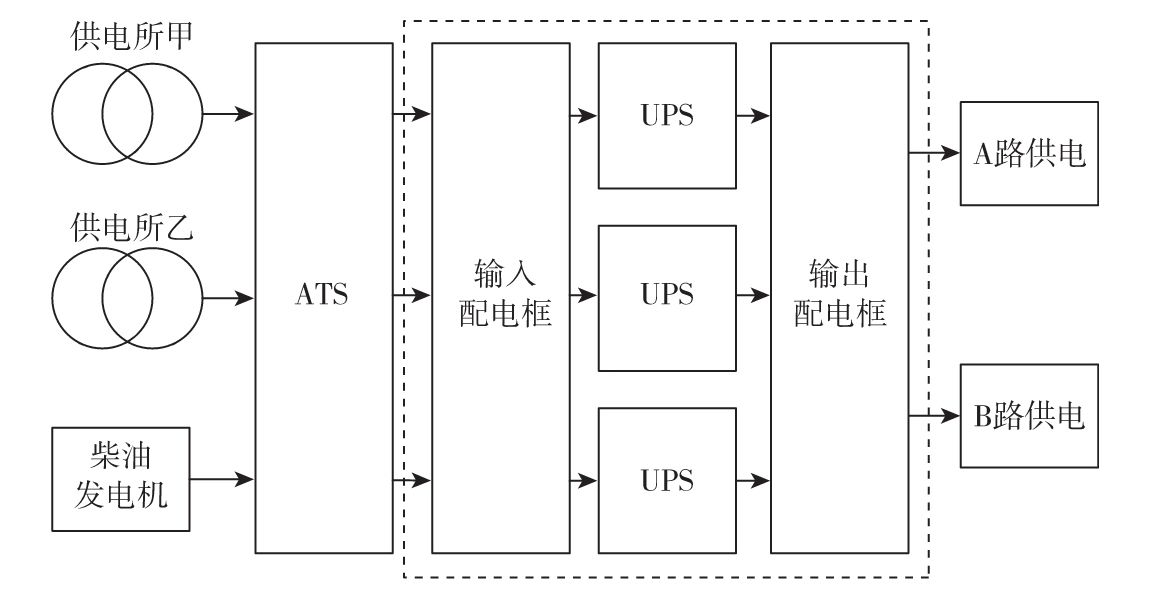
\includegraphics[width=1\linewidth]{1}
	\caption{供电系统简易示意图}
	\label{fig:1}
\end{figure}

我们对用电有三个基本要求——可靠、安全和容量。

1.可靠性要求

用电的可靠性要从如下几个方面来考虑。

首先,输电侧的高可靠性。输电侧的可靠性是重中之重,每年数据中心因停电引发的大面积宕机事件并不是个例。引入一类市电可减少类似事故的发生。

其次,全路径上的所有节点要保证充分冗余。说起冗余,我们作为运维人并不陌生,这也是老生常谈的话题了。所谓全路径,指的就是从输电侧到用户侧的整条输电线路。全路径上的每个环节都不能出现单点故障。这是一个逻辑与的关系,任何一处出现单点,整个系统的冗余就是零,跟没做一样。单条线路上的负载能力都应满足全部电力消耗总成,并留有一定的余量,一般应控制在80\%~85\%之间。在这里,经常会出现2N或N+X的概念。你可以简单地将N看成一个单点,2N就是双倍冗余,等效为存储中的RAID1。而N+X则是指,在多组节点中灵活配置的若干冗余,即可以看作RAID中的Spare盘。

再次,就是备用方案的持续支援能力。一旦主线路失效,作为最后一道防线的备用方案,除了切换及时以外,还要有强大的持续支援能力,以应对主线路无法及时修复的情况。例如我们前面提到的天津港大爆炸,它所引发的断电故障在短时间内肯定是无法恢复的。此时的首要任务是进行切换。假设极端情况下切换失败,那就只能靠备用方案来扛了。

最后一点也很重要,基础设施的采购一定要选用知名品牌,这样才会更有保障。另外,选用产品的原则是求稳不求新。对于一些新兴的技术,即便它来自于知名厂商的产品,我们还是应当慎重选择。

2.用电安全要求

除了可靠性以外,用电安全也是同等重要的。供电设施在长期使用后,会因线路老化发生漏电和人员触电的危险。因此,对于机房低压配电系统要求采用TN-S系统。什么是TN-S系统呢?在详细解释之前,我们需要先了解一些电的基本知识,看一看人体触电是怎样形成的。

电流和水的特性非常相像。常言道“人往高处走,水往低处流”,电流也是从高向低流动的。这里所说的高和低指的是电势。我们人为地将大地的电势定义为0,平时大家所说的××伏电压,指的就是输电侧相对于大地的电势差。除此之外,电流还有一个特性:如果遇到多条可以流经的路径,那么电流中的大部分电子总会选择电阻低的那条路径通过,即常说的电阻和电流成反比。这和我们平时开车是一样的。电阻意味着交通状况,谁都愿意走行驶通畅的道路。如果有两条路径,一条路径的电阻是1000Ω,另外一条路径的电阻是9000Ω,那么这两条路径上面的电流比则是9∶1。
发生触电需要两个条件。首先要具有电势差,其次要形成有效的回路。我们经常看到小鸟能站在高架电线上。那是因为鸟的双脚落在同一根电线上,而鸟的个体很小,两脚之间距离所形成的电势差几乎可以忽略不计,所以它们才能够安然无恙。但是,如果一个人不小心摸到了电门,由于人站在地面上,而大地电势为0,电流会因为电势差的关系,从输电侧经过人体流向大地并形成回路,这样就发生了触电。

为了防止发生触电危险,需要实施接地防护。以电源插座举例,插座面板上的三个孔分别为:左零,右火,中接地。火线(相线)是从输电侧引出来的线。零线(N线)由变压器二次侧中性点引出,用于和火线形成回路。电力在进入用户侧之前,由三根各成120°的相线组成。理论上,三相之间应当是平衡的。此时N线不带电,但这种状态不可能一直保持下去。三相失去平衡时在N线上会产生电流,所以N线必须接地,否则当其断开时会发生触电危险。地线是直接接地的保护线,我们称之为PE线。因为PE线的电阻非常小,相较几千欧姆的人体电阻来说要小得多。一旦人体触电,大部分电流会被它引走,从而确保人员的安全。PE线和N线的接地形式不同。PE线是从变压器中性点接地后引出主干线,并每间隔20~30m重复接地。N线则是在变压器中性点处与PE线重复接地,从而起到了双重保护的作用。

所以,接地是保证用电安全的主要手段。这里产生了一个有趣的问题:既然PE线和N线都要接地,那么如果我们把两股线合并在一起,岂不是节省了一大笔钱吗?这种系统就叫作TN-C系统,我们把这段合并的线称作PEN线。使用TN-C系统可以降低成本,但是它存在一些隐患。当PEN线路受损折断后,断点后端的设备金属外壳都会带电,此时如果有人不小心碰到就会触电。TN-S系统的PE线和N线是完全分开的,安全性高了很多,当然成本也就随之提升了。因此在实际生活当中,人们大多采用折中的TN-C-S系统,即起始路径采用两线合并的方式,在入户之前将PE线和N线分开,而且不允许再次合并。

根据国际电工委员会IEC的定义,供电系统分为三类(五种)——IT、TT、TN(包括TN-S、TN-C、TN-C-S),具体解释如下。

(1)第一字母表示电力系统的对地关系

·T——中性点一点接地。

·I——所有带电部分与地绝缘,或一点经阻抗接地。

(2)第二字母表示装置外露可导电部分对地关系

·T——外露可导电部分对地直接电气连接,与电力系统的任何接地点无关。

·N——外露可导电部分与电力系统的接地点做直接电气连接(在交流系统中,接地点通常就是中性点),TN系统后面还会有第三个字母。

(3)第三个字母表示中性线和保护线的组合关系

·S——中性线和保护线是分开的。

·C——中性线和保护线是合一的(PEN线)。

现在大家明白了吧。PE线和N线分开与否,以及接地点的数量决定了安全等级和成本的高低。尽管选择TT系统更加安全,但它的成本过于高昂。建筑物内如采用TN-C-S系统,其前段PEN线上的中性线电流所产生的电压降会产生电势差,对设备造成信号干扰。而TN-S系统适用于内部设有变电所的建筑物。因此我们要求机房内的低压配电系统必须采用TN-S系统。

除了人员的用电安全之外,我们在选取机房的过程中,还要注意静电对设备的危害。以下这些内容是我们在实际机房选型中对接地和防静电提出的一些要求。

·机房接地系统必须满足人身安全及运营设备正常运行的要求。

·机房内所有设备的可导电金属外壳、各类金属管道、建筑物金属结构等均应做等电位联结,不应有对地绝缘的孤立导体。机柜应有两根不同长度的连接导体就近与等电位联结网格连接。

·机房所在大楼的接地电阻应小于1Ω。

·等电位联结网格应采用截面积不小于25mm2的铜带或裸铜线,在防静电地板下构成边长为0.6~3m的矩形网格。

·机房地板或地面应有静电泻放措施和接地构造,防静电地板或地面的表面电阻应为2.5×104
~1.0×109Ω,且应具有防火、环保、耐污、耐磨性能。

\subsubsection{运维故事3:两路电}

“唉,邮件又来了!”最近管理员小王有点烦。一周之内,这已经是他第三次收到数据中心张小姐“善意”的邮件提醒了。大意是说,小王公司的300多台服务器一直采用单路用电(我们专业的电源策略应当叫作Redundant)的策略,导致数据中心机柜的A路高达18A(最高供电20A),而B路却是空载的。张小姐极力“建议”小王把现有服务器调整成两路均衡(Not Redundant)的模式。小王心里不太高兴,因为服务器默认出场配置都是冗余模式,又没有超电,为什么要我修改呢?刚刚休假回来的师傅老王听说这事儿以后,不一会儿就把所有服务器的电源策略调整为非冗余模式,并且给张小姐回复了一封邮件,告知其已经修改完成,同时对对方的提醒表示感谢。小王有点儿想不通,经过师傅的一番指点后终于明白了。“小王啊,人家机房建设多年,都像你这样高负载地总用一路,长期下来线路老化得快啊。张小姐一再催促你,她肯定是怕万一出了事儿,自己担不起责任。这就跟像穿鞋一样,两双鞋换着穿肯定比只可着一双穿要强。两路均衡的使用方式还是比较环保的,再者说改个电源策略也很简单。你要学会相互体谅,理解万岁嘛。”

3.电力的容量要求

电力容量是另外一个要关注的内容。容量选择和服务器选型有很大关系。以北京为例,一个机柜的年租用成本在几万元到十几万元不等,如果采购数量很大,这笔费用是相当可观的。因此提升机柜的利用率,是直接降低成本的有效手段。作为主数据中心,我不推荐采用20A以下的机柜。这样的话,空间利用率不会超过70\%,甚至会更低。企业规模越大越倾向于高电机柜的选择。如果当地电力设施条件允许,40A以上可能是最好的选择。以笔者实际工作中的测试数据为例,单台1U服务器的电流平均值常年维持在0.8~1A,峰值不超过1.3A。这样算起来,40A可以部署30台左右的1U服务器,再加上网络设备,无论是空间还是电力容量都实现了高利用率。PDU插座的数量要和电力容量以及上架设备的数量相匹配,并且应当留有独立于机柜PDU线路的插座,以供显示器、能耗仪等外接设备使用。而外接设备不应当直接接入生产的PDU插座,以防止因外接设备自身问题导致的电力故障波及生产。另外,我要提醒大家注意的是,PDU插座制式要符合国标。英制插座(俗称大头)在如今一些数据中心里还是能够看到的。

\subsection{空调系统}

空调的主要作用是降温和除湿,要想研究好空调系统,首先要搞懂气流。

说到气流,它可是一门挺复杂的学问。空调系统将空气进行制冷后,由风机送出冷空气,在与热源进行冷热置换后,达到降温的效果,经过置换后的热空气还要回流到空调系统再次进行制冷,如此周而复始反复循环。

那么要想达到好的制冷效果,控制好风速和风压是十分重要的。风速和风压是一个定值,它们是由设备机组决定的。我们这里把风压称为全压,全压总共由动压、静压和损耗三部分组成。气体在流动中会产生动能,这个动能所转化的压力就是所谓的动压。动压的大小和速度是成正比的。由于冷空气从风机里刚吹出来的时候速度快、动压大、气流不稳定,这些因素都会导致损耗增加。根据能量守恒定理可以得知,损耗越多,制冷效果肯定就越差。所以系统中都需要使用静压箱来减少动压、稳定气流,它可使送风更加均匀,从而提升制冷效果,同时还有降噪的功能。

电力和空调两大系统可谓是数据中心的任督二脉。甚至于有人这样讲:数据中心的核心就是管线和气流。然而它们却是一个看不见,一个摸不着。表面文章谁都会做,但真正的秘密其实都隐藏在那些看不见的地方。

\subsubsection{运维故事4:地板下面的秘密}

老张最近忙着数据中心扩建的事。招标书刚发出去没两天,各大数据中心的销售纷至沓来,可真是快把他办公室的门都挤破了。这不,今天老张又被一家数据中心请去参观。接待老张的是销售经理Cindy和售前技术经理Eric,一番寒暄后,先是由Cindy介绍了一下公司的情况,接着在Eric的引领下,大家一同去实地进行了参观。整个机房内窗明几净,整齐划一,布局合理,标准规范。老张看了看,不住地点头:“贵公司的数据中心建设得非常规范,简直可以做样本典型了啊。”

“哎呀,你过奖了,如果你觉得满意,我们在价格上还可以给你一个更加优惠的方案的。”Cindy听到老张的赞许,迫不及待地插话进来。

“不过,能不能掀开几块地板让我瞻仰一下?”

Eric微微一笑,“请你稍等”,说罢便转身走出了房间。不一会儿Eric一脸为难地进来了,“抱歉啊张总,实在是不太凑巧,掀地板的地吸被工人拿去施工了,你看……”

“不妨事,要不我们直接去工地瞧瞧?”老张不动声色地说。

“哎呀,你是大领导,工地乌烟瘴气的,怎么好亲下现场呢?我们去会议室休息一下吧。”Cindy也在一旁劝说。

“哈哈,算啦,今天也不早了,我也该回去了。整体来说确实不错,我回去向老板做个汇报,具体的我们会认真考虑的。”

一行三人来到大门口,临别前Eric不断地恭维着:“张总你可是老前辈,这次和你交流,我也是长了不少见识呢,回去之后还有劳你多多美言啊。”

“哪里,哪里,Eric老师你也是个中高手啊,哈哈。”

这番对话在Cindy看来,不过是两个人在相互恭维的商务礼节而已。但她却没有注意到,Eric说这话的时候,他脸颊上的微红与额头沁出的汗水。

1.送风模式

送风模式根据送风出口的位置主要分为两种。

第一种是上出风模式,如图2-2所示。它类似于日常生活中的空调系统。由于其送风方向和冷空气下沉的特性相一致,因此它的局部范围制冷快、效果好。此外,上出风模式还有不易产生积灰、设备问题易排查、扩建方便等诸多优势。然而它的缺点也非常明显,因为热空气往上走,而冷风往下送,送风方向和空气流动特性相悖。也就是说,这两者相互“顶起了牛”,使得机房的最下部区域的温度相对偏高。另外,由于屋顶的空间有限,对于进深比较大的机房需要增加送风管来保证送风的均匀,噪声也相对比较大。在承受辐射和寒冷的基础上,如果再加上噪声,这种环境对于在机房中长期工作是不利的。

\begin{figure}[htbp]
	\centering
	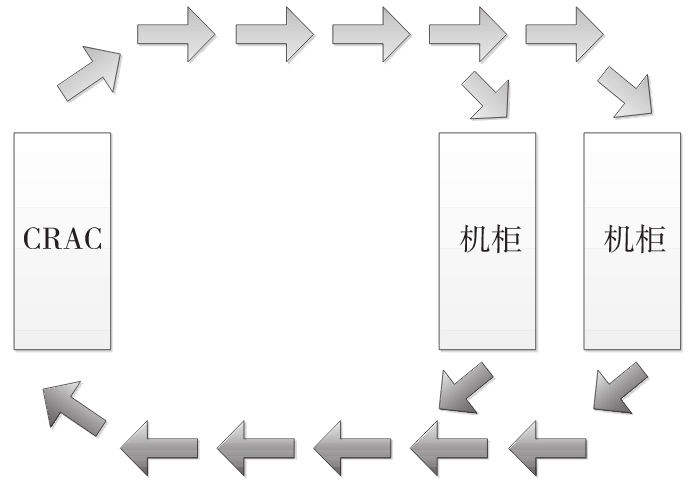
\includegraphics[width=1\linewidth]{2}
	\caption{上出风模式}
	\label{fig:1}
\end{figure}

第二种是下出风、侧回风模式,如图2-3所示。这是现今大多数新型机房采用的送风模式。因为下出风顺应了空气流动的特点,而且地板下方空间所构成的静压箱要比风管的横截面大得多。因此同等条件下,下出风的整体送风更均匀,温差更小,制冷效果更好。而且施工简单,无须风管和送风口。但下出风也十分考验地板材质、施工质量和布局的合理性。如果产品或施工质量不合格,会因为漏风出现送风短路。再有,地板下面容易积灰。防尘做不好的话,风机一启动就是漫天飞尘。建筑的层高不足,也不应该强行使用下出风的模式。因为活动地板空间有限(例如高度<400mm),后期扩建时的管线增加,肯定会影响到送风效果。还有,由于管线被埋在地板下面,不利于故障排查。这些都是前面故事里提到的地板下面的“秘密”了。

\begin{figure}[htbp]
	\centering
	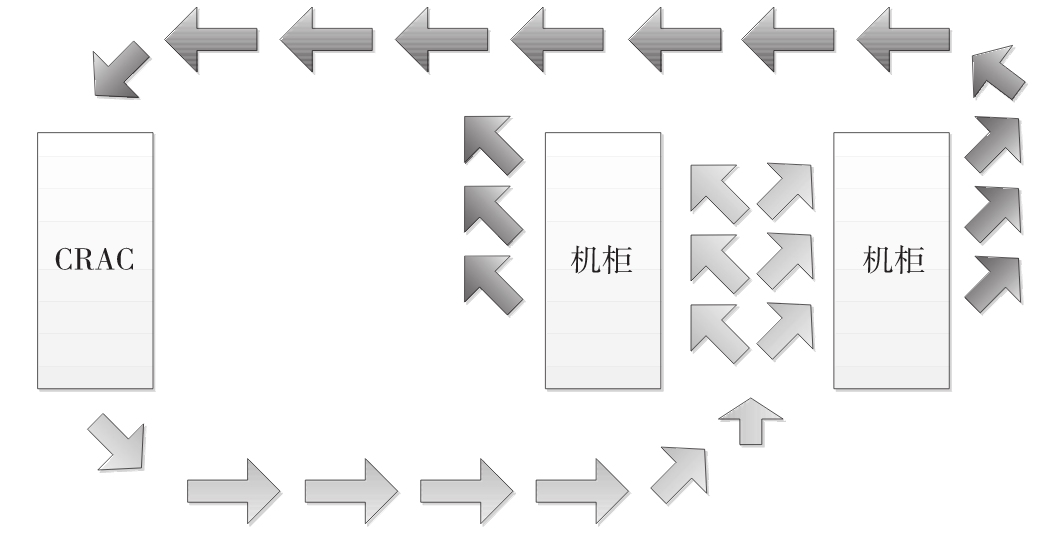
\includegraphics[width=1\linewidth]{3}
	\caption{下出风、侧回风模式}
	\label{fig:1}
\end{figure}

我们观察地板下的施工情况时,可采取一些简单方法。看走线是否规范,管线空间是否足够,布局是否合理,防尘保温做的是否到位,等等。具体指标可参考国家的标准规范,里面都有明确的指导。我们这些行外人不可能做到一一深谙其道,但至少你可以找到几条便于理解和判断的标准,暗暗牢记在心,到现场有目的地去考察。另外,可以多咨询一些专家,还要多看多问。其实很多知识往往就是在技术交流的过程中慢慢学习并理解的。

服务器风扇如果吸入的制冷量不能满足要求,会产生局部过热的现象。大数据的应用和强调高性能计算的今天,很多企业在选购服务器的过程中,也在大量选用高性能CPU和大容量磁盘的硬件配置。大功率和高密集型服务器的出现,已经向传统制冷提出了新的挑战。

为了保证充分有效地冷热交换,使用更高功率的风机显然是不节能的。而水平送风技术为我们提供了一种新的解决方案。水平送风的架构是制冷机组紧贴机柜安装,由多组风扇将冷空气水平送出,之后被吸入服务器,完成冷热交换后,再由服务器风扇排出,彼此之间就形成了一个有效的气流循环。尽管水平出风在我国并未真正普及,但这个思路还是值得我们学习和思考的。如果这种方式和下出风模式相结合,也许在不久的将来就会广泛地应用起来。

2.密闭问题

在机房里,我们经常听见别人谈论冷通道和热通道,顾名思义就是冷空气和热空气流动路径所构成的空间。以主流的下出风模式举例,我们看到现如今的机柜码放方式都是采取“面对面、背靠背”的策略。两个机柜正面之间的夹道就是冷通道,冷空气从通道下方送上来,从前方被吸入,再经置换后被风扇从机柜后方排出。而机柜背面之间的夹道就是热通道,热空气在此聚集后向上蒸腾回流到机组当中。

一般人们认为只要有足够的制冷量,使得温湿度达到要求就万事大吉了。但却忽略了气流的重要性。制冷量、风速和风压都是设备给定的,是否能达到好的效果是由气流决定的。这就和系统的性能调整一样,升级硬件也能解决问题,但如果不解决关键因素,势必要付出高额的成本代价。
关于密闭,我们刚才强调了地板下施工的问题,而在机柜这里也是一样。为了确保制冷效果,我们应当像静压箱的处理方式那样,对冷通道进行密闭。也就是对模块(两排面对面的机柜所形成的一组集群)通道的两侧加装安全门。除了起到封闭冷通道的作用,也增加了门禁的安全性,这已经是一种很普遍的做法了。讲到这儿,大家应当明白:送风短路(漏风)是制冷的大忌。所以我们时时刻刻都要考虑一件事,就是消除任何有可能发生破坏气流的因素。

第一,空闲机柜的影响。

假设一开始我们采购一个模块,但并不是所有的机柜都加电使用(因为加电意味着正式使用是要付费的),而是随着设备采购,逐步地开放机柜使用。空闲机柜如果没有加装盲板,由于空机柜没有设备,灌入的冷空气既没有参与热交换,也无法有效地形成回流,破坏气流平衡,造成能源损失。

第二,托盘上架方式。

我刚入行那段时间,接触过一些企业的内部机房。当时设备上架,像小型机这种贵重设备都是导轨上架,而x86服务器为了省事儿,都是直接将设备安置在托盘上的。托盘的种类分为两种,有上螺丝的,也有插销式的。因为托盘拆装方便,又比导轨的通用性好,所以这种上架在早期还是很流行的,当时很多整机质量较轻的设备都用托盘。但是为了防止形变,托盘面板都比较厚,因此是不能实现设备紧密码放的。很多人都习惯在上架的时候,各个设备之间留有1U或者2U的空间。现在大多设备都是前进风后出风,风扇足以带走大部分的热量。所以没有必要再留有空余。这样做既无益于散热,又浪费了机架的利用率。因为托盘的厚度会挤占下面U位的一部分,托盘和设备之间会留下不足1U的空位,而这段空位无法上盲板进行密闭,非常影响气流循环。现代数据中心采用托条来完成上架工作。它既继承了托盘的通用性优点,又实现了设备紧密摆放的需求。而那些没有设备的空U位,则需要加装盲板实现机柜密闭。

第三,机柜设计问题。

比如机柜边缘或对接处有缝隙。像这种有先天问题的机柜最好敬而远之。如果已经不可避免,也可以采用密封条等手段来补救。

3.精密空调的选择

在充分满足机房安全的条件下,应尽可能地选择高效节能的空调系统。空调系统常见的有风冷和水冷两种方式。说到制冷,最难熬的莫过于炎炎夏季了。这个时期是用电的高峰,最怕的就是停电。风冷系统需要定期换气,从外部引入新风与回风进行混合。所以,水冷效果显然在夏季要比风冷更好,而风冷的效果在冬天会得到加强。当然,选用水冷系统要看实际的地理位置和使用年限。水冷的效果受到水质的影响,而且后期维护成本高,时间一长制冷效果会越来越差。如果你是新机房,水冷肯定是优先选择的。如果当地水质不好,或者制冷机组已经用了很多年,可能就要实地考察一下制冷效果了。水冷一般都会选择下出风,万一你真遇到了上出风的水冷,一定要考虑漏水是否会影响到设备的安全。

精密空调的安装位置也有讲究,应尽量靠近热通道和热负荷区域。在设备选型上,应尽量选择单台制冷量更大的设备,并且以显冷量作为主要衡量目标,而非全冷。这里涉及两个概念——显冷和潜冷。这两个概念是由热力学中的“显热”和“潜热”派生而来的。具体的含义就不做过多解释了。简而言之,我们知道空调有两个功能——温度调节和湿度调节。所谓显冷量是指降温时所需的冷量,而潜冷量则是指产生冷凝水所需的冷量。全冷=显冷+潜冷。而数据中心的首要任务是降温,因此在选型过程中应以显冷量作为主要衡量目标,以免低估了制冷量的需求。

精密空调的冗余方式为N+X。这里X的值我们推荐最好是2或3,太少可靠性差,太多浪费成本。关于N的显冷总量的设计,我们建议机房最大的总负荷值不应该超过显冷总量的85%。

4.气流组织

数据中心对气流组织的要求主要包括以下内容。

·冷通道内温度任意点均不高于24℃,热通道温升对比冷通道不超过12℃温差,避免通风量不足造成局部过热;针对高功率机柜散热,应通过增加通风地板面积、通风孔率,局部风扇地板,局部精密空调等方式解决。

·在空调因断电或其他因素停机或切换时,机房冷通道内温度不超过30℃;一般情况下,5kW机柜,末端空调恢复通风供冷时间不超过10min,8kW机柜,末端空调恢复通风供冷时间不超过6min,否则机房会出现规模过热的风险。

·板下送风气流组织,下送风应均匀,风速不超过3m/s;采用风道送风时,送风风速应满足相关通风风道设计规范,主干管风速不超过8m/s,支管风速为3~5m/s。

·送风距离:单侧送风距离应小于15m,大于15m应双侧送风。

\subsection{消防系统}

数据中心是耗电大户,因此必须加强防火意识。机房耐火等级不应低于二级。机房应当配备至少两个以上的安全出口,门的开启方向要和疏散方向保持一致,且在任何情况下都应当能够从房内开启,并完成自动锁闭。灭火装置应选用IG541或者七氟丙烷气体。表2-1是这两种气体的特性对比。

\begin{figure}[htbp]
	\centering
	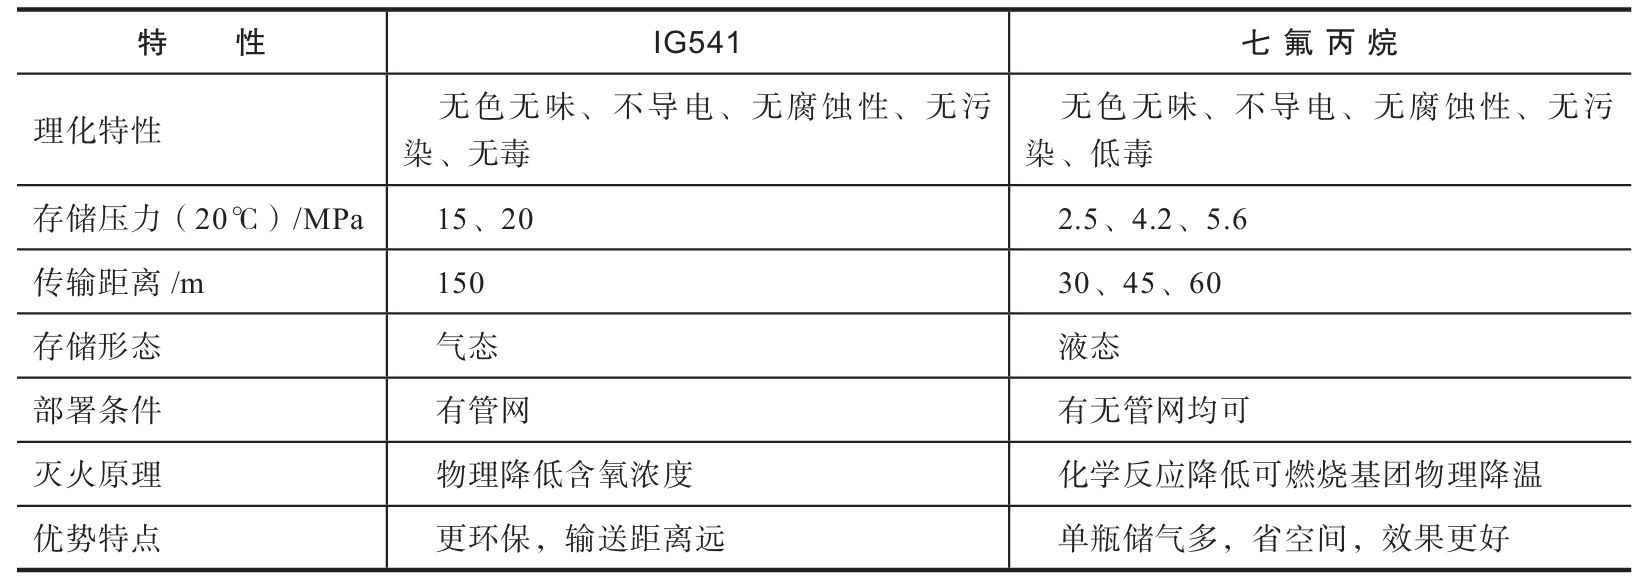
\includegraphics[width=1\linewidth]{4}
	\caption{IG541和七氟丙烷的特性对比}
	\label{fig:1}
\end{figure}

\subsection{弱电与综合布线系统}

弱电系统主要包括传感器监控、影像监控、门禁系统及入侵检测等。总体原则上只要做到无死角即可。除了空调机组自带的回风温度探头,在机房的每个冷通道内,至少头部、尾部和中间应各部署一个温度探头,在热通道内部署一个温度探头。每个通道两侧应各部署一个摄像头。

机房内应当有不少于两部可用于外拨的固定电话。通常,机房内是没有手机信号的,因此要部署固定电话,以便在遇到特殊情况时,能够直接和外界及时联络。

如果你比较关注机房的总体情况,例如能耗、温湿度等信息,希望能够将相关数据直接接入自己的监控系统,那么机房的监控系统需要支持类似HTTP、SNMP、TCP/IP等主流的通信协议。

综合布线的大致要求有三点:第一,强、弱电的线缆要分开,并且要注意它们之间的间隔;第二,线缆走线要平行无交叉,途经路径要注意规避潮湿、易漏水、易喷水等地方,该套管的地方要套管;第三,管线空间规格要符合标准,注意有可能折损、破坏线缆的因素。

以下这些内容是我们在实际机房选型中对综合布线提出的一些要求。

1)强弱电分离:机房桥架应满足强电线缆、弱电线缆、光纤等分开布放需求;一般情况下,机房应采用上走线、下送风方式,走线架宽不小于400mm,下层走弱电,上层走强电,弱电桥架内安装光纤槽道,强电与数据铜缆、光纤之间的间隔不小于200mm;当采用开放式走线架时,如果弱电走线架与强电走线架平行布置,则二者的间隔距离不应小于300mm。

2)光缆槽道:普通机架光纤槽深度100mm,宽度120mm,核心网络区域机架光纤槽深度100mm,宽度320mm,出线口要求不小于300mm。机房内所有机架要求普通光纤槽覆盖。

3)机房应保证提供双路由光缆接入条件,允许其他运营商光缆直接入局或与其光纤互通,并协助解决相关光缆接入事宜;具体光纤需求数量配置能满足按需扩容;当有到达同一站点不同路由的需求时,可通过迂回绕接来保证全程无路由重叠,光缆落地施工时务必尽可能走不同的管接进进机房。

4)光缆技术指标:线路光纤类型G.652,平均单位光功率衰耗常数≤0.5db/km;光纤色度色散系数应≤18PS/km·nm,偏振模色散≤0.2PS/km1/2。

5)连接可用性:丢包率不高于1\%情况下,保证连接可用性达到99.99\%。

\section{网络建设评估}

这里所说的网络建设,不是指具体的网络性能指标,而是指数据中心能够提供的网络资源与建设资质。数据中心的网络资源有专线和裸光纤两种。专线传输距离远,但租用价格高,带宽上有限制。裸光纤理论上带宽不再受限制,适合短距离、大数据量传输。同城多机房的各节点之间互通建议使用裸光纤。但拉裸光纤这种事吃力不讨好,造价高利润少,作为运营商,肯定是不会随便开这个口子的。如果这些节点不是同属一家数据中心,那么它们之间要实现互通,可能就更加困难了。这个时候你就知道,一个有着丰富人脉资源的数据中心经理是多么重要了。

前面我们反复提到过冗余问题。在全路径的各个节点上,都需要做好冗余结构才行。假设在北京,从东四环到南五环外路穿线。正常情况下,一条应该走四环,另外一条走五环才对。不能所有的线缆都走同一条路径。再如,铺设线缆应该进入正规的管井之中。如果承建商根本没有资质和资源,被管理部门拒之门外,最后只能把部分线缆甩在外面,也就是我们常说的“野纤”。野纤再加上单路径,其隐患可想而知。之所以会有这些问题,归根到底就是一个“钱”字。资质要花钱,多路径也要花钱。而这些工程隐患的出现,正是一味追求低价所引发的后果。

\section{服务保障评估}

可用性要考评数据中心的对外服务能力。据说,200个机柜对一个IDC运维来讲,他的工作将达到饱和状态。数据中心是不太可能提供过多的人员充分保证每一家用户的使用需求的。如果有7×24小时值守服务的特殊需求,应确保有专职人员服务,在合同需求中也要有所体现。如果数据中心保证不了,则需要另行招聘驻场人员。

\subsubsection{运维故事5:一山难容二虎}

销售经理Tina听说Forever公司要扩建新的数据中心,急忙和售前经理赶去拜访。她精心准备了几十页的PPT,不遗余力地为自己的企业进行宣传。当讲到服务客户这一页时,Tina显得很有自信:“我相信贵公司如果选择我们的服务,那将会给你带来更加有效的保障。因为我们正在为很多知名企业提供数据托管服务,例如Something、Balabala,还有……”

深谙市场行情的老D忍不住插了一句:“抱歉打断一下,我听说Never好像也在你们那里哦。”

“啊?呃,是的。”这个突如其来的问题让Tina显得有点儿不知所措,她刚刚才发觉到Forever和Never的竞争关系。

老D又补了一句,“我们的需求数量和Never在贵公司现已保有的数量相近,大家都是大客户,那么请问,如果出现资源争用的情况,你们会优先保证谁的服务呢?”呃,这句话没法接啊,一时间Tina自己都不知道该说些什么好。

\section{本章小结}

上述我们所讲的不过是数据中心的一些皮毛而已。具体的细节,大家可以参考以下这些规范(因书籍出版的时效性,请读者自行更新最新版本):

·《计算机场地通用规范》(GB/T2887—2011);

·《计算机场地安全要求》(GB/T9361—2011);

·《信息安全技术信息系统安全等级保护基本要求》(GB/T22239—2015);

·《数据中心设计规范》(GB50174—2017);

·《数据中心基础设施施工及验收规范》(GB50462—2015);

·《建筑物电子信息系统防雷技术规范》(GB50343—2012);

·《气体灭火系统设计规范》(GB50370—2005);

·《气体灭火系统施工及验收规范》(GB50263—2007);

·《综合布线系统工程设计规范》(GB50311—2016);

·《综合布线系统工程验收规范》(GB/T50312—2016);

·《视频安防监控系统工程设计规范》(GB50395—2007)。

最后我们总结一下考察机房的几点注意事项。

第一,便宜没好货。

在招投标里,商务价格往往占比很重。少数厂商为了中标,不惜赔本儿赚吆喝。然而,有些成本是省不了的。如果一味看重低价,甚至是不合理的低价。其结果势必会有两傻:要么乙方是傻瓜,赔钱做善事;要么甲方傻眼,到时候不是质量有问题,就是后续要产生费用增项。

第二,多看实际生产环境。

有条件的话,应当尽可能去生产机房参观。建议多在各个楼层进行走访,考察不应只停留在一个地方。

第三,不要只提问不回答。

项目实施最忌讳的就是沟通不充分。甲方往往容易犯一个错误——那就是提问多,回答少。甲方总是关心乙方能不能满足需求?你想有谁会说自己满足不了呢?需求讲不明白,细节方面落实不到位,对方又没能充分理解,就容易产生偏差。能不能做不是重点,需求有没有充分地表达清楚才是关键。

当然,最后还是要多多学习,扩展自己的知识面。

就像我开头讲的,可能公司没有那么多专职岗位,一些工作需要你兼职来完成。建议大家平时要多积累一些周边知识,做一名T型人才。

\chapter{数据中心的规划设计工作}

万丈高楼平地起。一个优秀的规划设计方案是一切良好的开端。数据中心的规划设计工作是分阶段的,并非一蹴而就。它的生命周期贯穿于整个项目建设的进程之中,我们可以依照时间点将它分成三个阶段。

第一阶段——准备工作

。在开始规划设计之前,首要的任务是完成设备选型和能耗测试。设备选型应依据业务需求而定,方案确定以后,才能据此展开能耗测试的工作。能耗测试的结果非常重要,它是计算电力容量和空间利用率匹配最优解的核心参数。由于各家数据中心的电力容量和机柜价格并不相同,根据最优解,你才能够进一步得出总体成本的最小值。因此,设备选型和能耗测试可以帮助我们找出那些符合预期要求的数据中心。

第二阶段——实地调研

。在入围采购的筛选过程之中,实地调研是必不可少的一个环节。在这个过程中,我们要关注实际情况与最初设计方案之间是否存在着一些偏差。如果这些偏差不是硬伤,那么这家数据中心就具有入围资格,未来也有中标的可能性。设计方案就要为此做出一些调整。比方说,为了确保网络链路的冗余,我们希望单排机柜的数量以偶数为佳,便于将来布局时采取两两一组的形式来分配机柜。如果实际情况恰恰相反,那么单个机柜怎么用就是你要考虑的事情了。因此,在调研时最好能够参阅数据中心的平面设计图。从全局的角度观察,能减少问题死角带来的麻烦。从这一点上我们也能看出,设计方案存在着动态调整的可能性。

第三阶段——平台建设

。在完成采购任务后,接下来就是进一步的细化工作了。这里的工作重点在于——设计方案要如何保证各个子系统之间的平衡。在规划具体的细节时,建议邀请网络和系统方面的一线工作者一同参与探讨,充分考虑他们在实际工作中的需求。此外,还要注意业务需求的多变性,它会带来很多不确定性的因素。

\subsubsection{运维故事6:计划赶不上变化}

眼看年关将至,信息中心新一年的机房设备采购计划再一次启动了。因为业务增长得太快,现有的机房已经不够用了。为了确保日常维护工作的正常运行,经过上级领导批准,已经同意信息中心走内部的续采流程。信息中心将和现在这家提供托管服务的数据中心再签订一份增补合同,把现在正在使用的306号机房旁边的308号机房也租用下来。新机房的规模和布局与老机房完全一致,就等各部门上报采购计划了。只要需求数量一落实,就可以确定二期扩容所需机柜的数量。

时间紧任务重,领导让新来的雷小虎负责本次统计规划的工作,要求各组负责人尽快上报自己团队的采购计划,把数量交给雷小虎汇总。过了一个礼拜,各组的数据陆续递交了上来。雷小虎看了一下数据清单,发现业务二组的数据还没有上报。于是,他赶忙去找二组组长老尤求助。

“尤组,上周领导吩咐我统计采购计划的需求数量,你看能不能安排个人配合一下?”老尤嘿嘿一笑,“这事好说,我让小米来支持你。”

“小米,你来一下。”

“领导,需要我做什么?”听到老尤的招呼,小米不敢怠慢,急急忙忙地跑了过来。

“中心需要各组配合申报明年的采购计划,你就负责配合小虎完成咱们组的任务吧。好了,具体的事请你们俩对一下吧。”

“好的,老大,我一定全力配合。”小米笑眯眯地连连点头。

“那就这样,一会儿还有个会,我先走啦。”说罢,老尤转身离开了。

小米看着老尤走远后,转过身来一副笑脸地对着雷小虎言道:“虎哥,关于这个具体问题呢,我也不太清楚。你看,我们日常工作也只是负责维护和项目对接而已,这个设备具体的使用方是国际业务综合办。说白了我们其实就是一个二房东,代人家提采购需求的。我看咱俩还是直接去找综合办的小胡问问吧。”

于是,两人找到了综合办的小胡。小胡介绍说,来年准备上一个新项目。因为综合办在四季度的走访调研过程中得知,一些用户反映社区业务的沟通渠道少,办事效率低。为了支撑社区工作开展,综合办决定设立一个论坛空间。但因为要给外网访问,不能和现有业务放在一起,需要单独隔离出来。大概需要五台服务器。

“只有五台啊,这可有点儿浪费呀!”雷小虎暗自嘟囔着。因为机柜都是两两一组,即便只用几台做隔离,也势必要挪出两个空机柜来。

“那你们以后会不会扩容呢?”雷小虎突然想到这个问题,有点不放心地又追问了一句。

“哦,这个应该不会吧。我看就算是扩容,也增加不了几台机器啊。”

“好,就这么定了,那我就写报告去了。”看着小胡信誓旦旦的表情,雷小虎天真地相信了。

又过了一个月,小胡领着小米兴冲冲地跑来找雷小虎。

“虎哥,上次咱们讨论的那个社区论坛的项目需要再增加50台服务器,你看能不能尽快给我们安排一下。”

“什么?再加50台?你们不是说不会再扩容了吗?怎么会又多出来这么多需求?”

“嗨,原来我们以为增设论坛只是为了满足一部分人的需求,所以就没太在意。没想到这个论坛一上线,立刻就引起了很大反响。很多用户打来电话,说除了论坛希望能再增加一些什么短信提醒、邮件反馈之类的功能。用户热情高涨,领导说这个项目要加大投入,所以我们的需求就变多了。”

“可是你们这个项目是需要做隔离的,当初就作为一个特殊需求,没有预留那么多的地方啊?”

“那咋办?我们现在很急啊!领导现在是亲自督办此事,不能耽误啊。”小胡一脸不高兴的样子,转过身来问小米,“你就说我们现在去找谁吧。谁能解决这个问题?”

“你……”雷小虎不知道该说什么好。综合办是业务部门,在单位里那可是一线明星部门,很有话语权。而小胡一看事情不好办,有可能要耽误她的工作,脸立马就拉下来了。这种瞬间的态度变化让耿直的雷小虎有点儿接受不了,尤其是她那动不动就搬出领导压人的姿态更是让人觉得不爽。

小米在一旁开了腔,“据我所知,咱们不是还有空闲的机柜吗?”

“空机柜倒是有,可是那些都是我已经规划好了的呀。”

“但是你现在也没有别的办法呀。我们先临时借用几个,到时候买了新机框再还你几个不就行了嘛。唉,项目进度重要啊。”

“就是,就是。到时候我们加倍偿还。嘻嘻。”小胡也在一旁打趣到。

“你们知道什么,这又不是借橡皮,使完了还回来就行了。”这句话雷小虎嘴上没说出来,但心里很不痛快。借出去的机柜哪有原封不动地归还的,不过是拆了东墙补西墙罢了。虽然数量上是没有亏损。但是原来整齐的规划排序就全乱了。本来他已经将不同的区域都用颜色标识给规划好了。这样来回一折腾,计划好区域就打散了。好好的彩色规划图,弄得就跟马赛克壁纸一样。以后管理起来还是个大难题呢。

两周之后……

综合办的老白也来找雷小虎。

“小虎,我们最近又有一个新项目,需要50台服务器,而且要和现有项目隔离。你给看看怎么弄?”得,麻烦又来了。

“白哥,你确定就是50台,你们还有没有扩容了?”

“这个我可说不好。你就先来50台吧,到时候不够再说。”

“白哥,都这么弄我可有点儿掌控不住啦。你不提前规划好,我不能总是东拆西借的啊。”

“扩容这事儿我哪能知道啊?我又不是诸葛亮能掐会算的。我现在就要50台,其他的以后再说。”话没说两句,老白反倒先露出了不耐烦的神情。“那好吧,白哥,我先去趟洗手间,回来咱们再商量。”说罢,雷小虎阴着脸走出了办公室。他哪里是上什么洗手间,现在的他气血上涌,只想找个地方一个人静静。

\section{需求的不确定性}

规划最怕的是变化。变化是我们在规划设计中遇到的最大的阻力与麻烦。问题的根源就在于需求具有不确定性,它就像是测量学中的误差一样不可避免。很多项目变更的出现,正是因为前期需求没有讲清楚造成的。“讲不清”的主要原因有两个:一个是“说不好”,另一个是“没想到”。这种问题在那些新项目中尤为常见,特别是在创业公司或者业务转型的时期及其普遍。

开展一个全新的业务,存在着很多不可预知的因素。我们对于新业务的整体运作是抱有试水心态的。大家都知道“小马过河”的故事。虽然在过河之前,小马通过调研的方式对可行性进行了充分的论证,但它毕竟没有实践经验,所以在迈出第一步时,是没有十足把握的。同样,新项目上线后,你并不能确保它就一定朝着理想的状态发展。这是一个尝试的过程。如果顺利,投资力度自然就会加大。反之,业务就会缩减甚至取消。

从这个逻辑角度上来讲,业务部门在很多情况下是没办法预测需求的。我们发现了一个有趣的现象,预估的需求量总是小于实际的需求量。这是因为申请人采取了保守策略的缘故。人们常说“不要把弓拉满”,采取摸着石头过河的方法,其实就是为了给自己留有一些余地。但不管怎么说,项目成功的可能性更大一些,所以增项变更是大概率事件,我们必须为此要做好一些额外的准备。如果你处理不好这种问题,将会给后续工作带来非常大的麻烦。

\subsubsection{运维故事7:续采之怒}

“他严涛到底是什么意思?这分明就是在耍我!”采销科主任刘致远把桌子拍得啪啪直响。一看老大发了脾气,科室里面的人一个个全都低着脑袋不敢吱声,生怕这倒霉的无名之火烧到自己的头上。

“这个采购单我刚刚结束还没有一个月,他又来提交续采申请。难道他不知道这种事情在审计那里是通不过的吗?”

单位有明文的规定,所有采购项目必须招标,是不允许直接采购的。当然,有的时候为了保证项目运行的连续性和可靠性,在说明理由的情况下也可以申请续采。但是,这次项目采购刚刚结束,供应商尚未供货。在这个时间就去提续采申请,审计显然是不会给予批准的。如果非要续采,意味着刘致远必须重新开启一轮新的招投标,相当于一件工作做了两遍。即便这样,审计处的人照样也会找他的麻烦,一定会问他什么要提两次采购需求。当然,他严大主任只是替国际业务综合办的老白提采购需求而已,他要的就是进度,其他事情他是不会关心的。所以刘致远觉得自己平白无故地背上这口锅实在是很憋屈。

就为这事儿,俩人在例会上针锋相对地大吵了一架。本来这事儿确实是不太正常,但各部门都有自己的理由,而且综合办的政治地位在单位里那是数一数二的。最后业务、审计、采销部门的几个高层领导一商议,批示如下:请采销科着手速办,请审计处绿灯放行。一切以业务为重,这种情况下不为例。

下不为例?鬼才相信呢。在刘致远看来,姓严的根本就是不负责任。像这种情况不是一次两次了。前期需求没搞清楚,出现了变更之后,也不和自己提前沟通一下,先斩后奏地搞突袭,最后再让综合办的人出面给他施压。再这么下去,以后的工作真是没法干了。

\section{如何避免变化打乱规划}

既然需求变更是不可避免的,那么提前预判并采取积极有效的应对措施就显得十分重要了。假设我们将需求比作一只吹满了气但没有扎口的气球,一旦松手,这只气球会到处乱飞,毫无规律可言。而规划设计就像是四周的墙壁,它会限定气球的飞行。如果墙壁合围的空间过小,气球在飞行的过程中就有撞墙的可能,这就代表需求和规划之间产生了冲突。如果我们能事先评估,尽可能地将所有的飞行路线都考虑进去,并为此预留出一些空间,那么冲突的概率就会降低很多。

\subsection{采购资源预留}

比如说上面这个续采的例子,业务部门是设备的使用者,但是设备资产和管理是算在IT部门头上的,所以IT部门要负责提交采购申请。这里就存在很多矛盾。东西不是我用,但我要负责提采购需求,而采购需求又说不清,怎么办?大额采购的周期是比较长的,不可能让你频繁下单。但预留太多资源,财务又会削减你的预算支出。假设业务部门计划采购50台设备,你在此基础之上又预留了50台。财务部门在审核的过程中,可能会对业务部门进行调查。业务部门原本就认为自己只需要50台设备,在面对挑战时,没准儿还会缩减最初的计划。此时,这100台的设备采购预算肯定要遭到削减。

从这个例子上可以看出,资源预留不能闭门造车,必须和业务方进行充分沟通,就各种风险及解决方案达成共识。

首先,技术部门要提醒业务方,后续有可能出现增项变化。然后针对这一风险,给予对方一个合理化的预留建议。比如把设备数量从50台改为70台。

其次,要注意需求有失控、超出预期的风险。如果预留资源在未来无法满足增项需求,我们将面临着两种抉择:要么砸掉原有的墙壁继续扩容,要么让气球停下来。无限扩容显然是不现实的,好的做法是拆解超出范围的那部分需求。假设设备增项是50台,我们看一看在这50台里面,能不能把最紧急、最重要的先安排进去,其余的挪到项目二期去完成。

最后,还有一点要特别注意:在后期的扩容工作中,你要考虑是否存在迁移、停机等一系列问题。把这些内容明确下来,让业务部门有充分的心理准备,双方要就此达成共识,这一点非常重要。

\subsection{数据中心机柜区域的规划与布局}

设备的上架与迁移,在数据中心的日常工作中乃是家常便饭。如果前期没有一个合理有效的规划,加之人员变动频繁、岗位交接不清等因素的影响,日久天长容易出现资产混乱的问题。

古人云:一室之不治,何以天下家国为?机柜区域的规划与布局可是很有讲究的。你可别小看它,一个合理、高效的规划布局,不但能最大程度地提升空间利用率,节约项目开支,同时还具有很强的视觉效应。如果方案设计得合理,你完全可以将整张平面规划图清晰地印在脑海之中,便于理解和记忆。那么,日常的管理工作就会变得更加轻松。反之,如果你走到一处,都不清楚这里是干什么的,工作效率想必也高不到哪儿去。

按照应用的角度划分,我们可以把整个空间分为三个部分——生产区、非生产区和基础设施。生产区的设备均属于线上系统,只能由运维团队来管理。非生产区则主要用于开发和测试的工作。它对可用性的要求不高,但对自主操作的需求非常强烈。所以,非生产区的权限可以更加开放一些。由于开发和测试本身就有不确定性,在使用过程中会带来一些破坏,因此非生产区与生产区之间必须实施隔离管理。这里有物理隔离和逻辑隔离两种形式。前者需要在网络的拓扑结构上进行隔离,后者则可以通过防火墙来达到目的。数据中心的基础设施不作生产与非生产的区分。生产区和非生产区都有各自对应的基础设施,你可以将它们分别放置在不同的机柜里以示区别,但它们应当依旧同属一个空间。

接下来,我们还可以将这三个空间进一步细分成九种不同类型的区域。详细情形如图3-1所示。
下面,我们分别介绍这九个区域。

\begin{figure}[htbp]
	\centering
	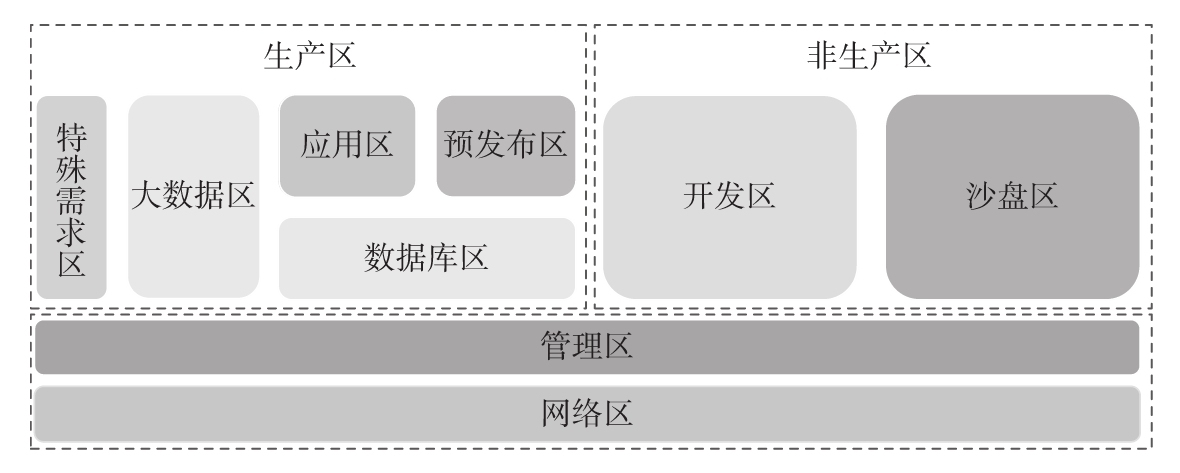
\includegraphics[width=1\linewidth]{5}
	\caption{区域分类}
	\label{fig:1}
\end{figure}

(1)网络区

顾名思义,网络区主要用来安置核心层的网络设备,以及与银行对接的一些专线设备。该区域的Owner为NE(网络工程师)。

(2)管理区

管理区用于提供维护管理功能,它涵盖了所有的基础服务。例如,部署系统、资产系统、DNS、文件共享、配置管理、监控系统、安全检测系统等。该区域的Owner为运维团队的所有成员。

(3)数据库区

数据库区用于安置数据库服务器。当然,你可以根据实际情况再做细分。例如,根据数据库类型来划分(Oracle、MySQL等),或者根据业务等级来划分(核心数据库、普通数据库等)。如果数据库需要外接存储,则需要综合考虑存储的空间占位与能耗,带存储的数据库最好和不带存储的数据库分开安置。该区域的Owner为运维DBA。

(4)应用区

应用区用于安置前端应用服务器。它通常位于网络拓扑的DMZ区。应用区是设备数量最多的区域,同时也是变数最多的区域。这需要你事先预留出充裕的空间。该区域的Owner为PE(产品工程师/应用运维工程师)。

(5)大数据区

由于对计算能力和存储空间的要求很高,大数据服务器的能耗非常惊人。以Intel E5-2640v3加12块4TB磁盘为例,350W的整机能耗只能算正常值。如果计算任务比较繁重,则其峰值会更高。所以大数据服务器不可以和一般机型混放在一起。为了提升空间利用率,建议你为数据节点服务器选用电力容量更高的机柜。名称节点服务器等其他设备和普通服务器相比,则没有太大的差别。你可以考虑在大数据区内部划出一块地方,专门安置它们。

(6)预发布区

预发布区属于准生产区域。研发和运维是两个体系,生产系统不允许研发人员直接操作。产品代码在完成测试之后,都是交付给运维团队负责上线的。测试环境和生产环境之间可能会存在一定的差异。如果上线发布后出现异常,则需要回退操作。代码有问题是很常见的,回退操作将严重影响系统的可用率。而预发布区可用于模拟线上的真实环境,进一步保证了生产系统的安全更新。

(7)特殊需求区

特殊需求区主要用于承接各式各样的“非主流”需求。例如,构建特定的隔离环境、安置非标准配置的服务器、临时迁移或借调设备等,这些特殊情况都不适合做统一的安置。此时,你可以把它们统统都放置在这里。我把它也戏称为“奇葩需求区”,意思是:不管你提出什么千奇百怪、偏离常态的需求,我这儿都可以满足。这个区域的空间应当多预留一些。如果用不完,后期可以慢慢回收。我的原则就是:你可以乱,但只能乱一点儿。一定要把维护成本限定在可控的范围之内。

特殊需求区的安置位置是有讲究的,建议放在应用区和数据库区的中间。另外,它的使用方式也有所不同,应当从中间的机柜向两侧扩展使用。因为要应对“需求气球”的变化,一开始会预留很大的空间,随着应用、数据库服务器的不断增加,这个空间会被逐步压缩。这种安置和上架的方式,体现了较强的灵活性,可以从容地应对未来有可能发生的需求数量的变化。

(8)开发区

开发区主要面向研发和测试人员。如何定义开发区的空间大小,这取决于团队规模和产品种类。理论上,开发区在业务扩张时期的需求量最大,但不会无休止地增长。由于开发产品的团队很多,为了防止干扰,开发区内部也存在着逻辑隔离的需求,我们通常管它叫闭环系统。

(9)沙盘区

沙盘区用于实验论证,它是为新技术探索研究或者故障复现而设立的。沙盘区不需要预留很多,一般不超过六个机柜。但它会带来比开发区更多的风险,所以沙盘区必须实施隔离。

\subsection{规划布局案例}

说了这么多,我们来举一个规划布局的实际案例。如图3-2所示,这是某个数据中心的机房平面局部图。

\begin{figure}[htbp]
	\centering
	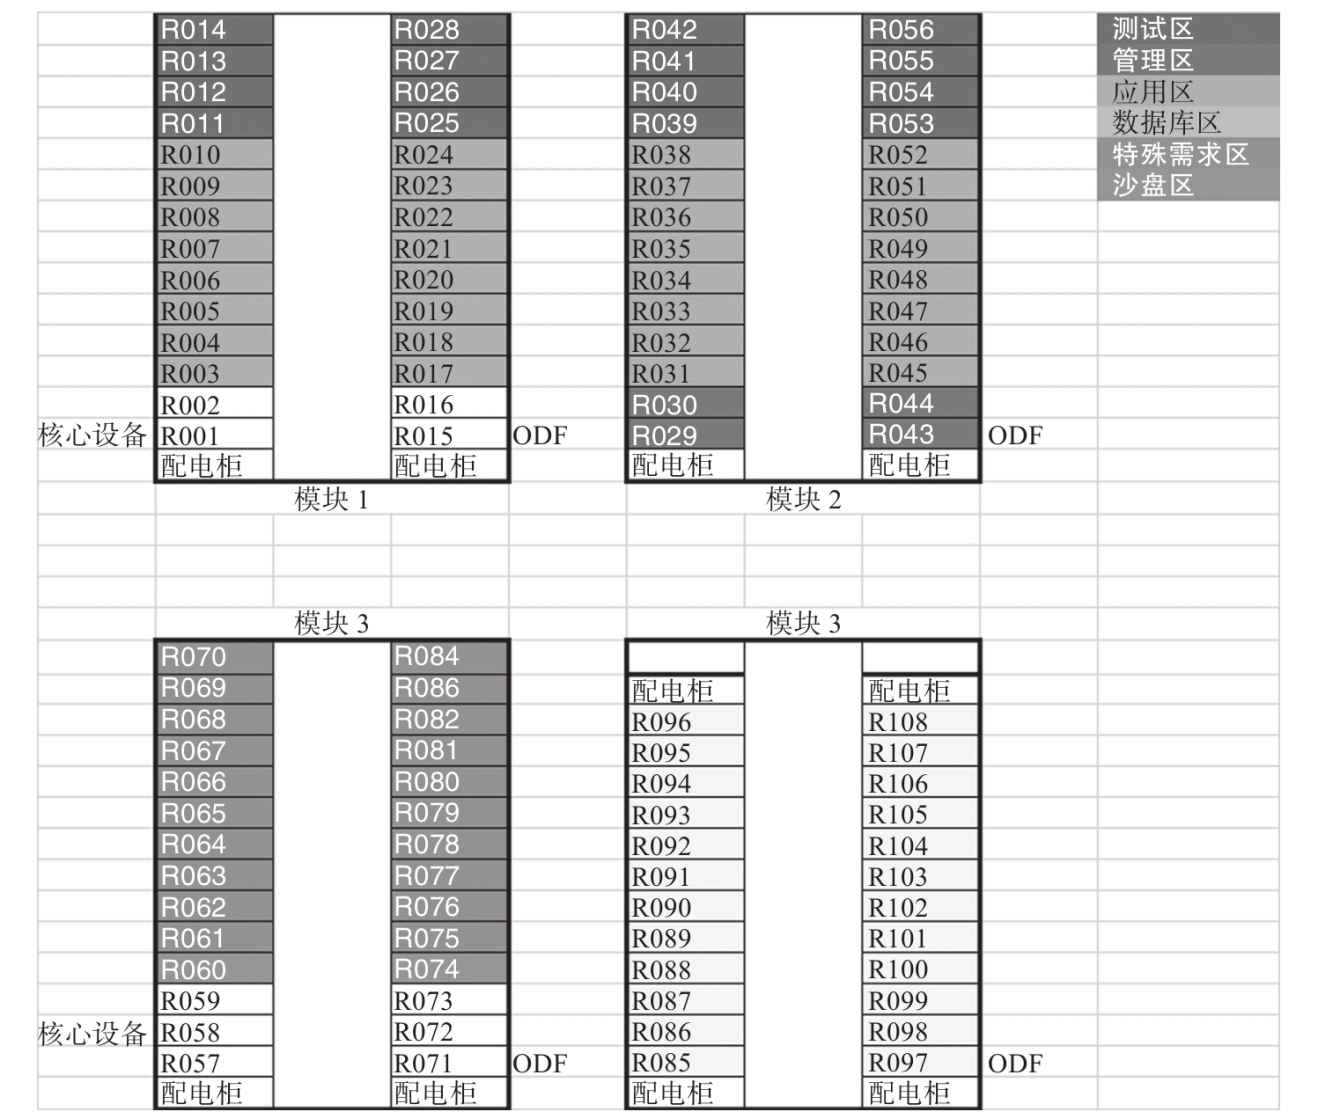
\includegraphics[width=1\linewidth]{6}
	\caption{区域规划案例}
	\label{fig:1}
\end{figure}

模块3中的核心设备即网络设备。部署网络设备应尽量靠近列头柜、配电柜等基础设施,还要注意对线缆长度的影响。穿线路由与线缆距离可通过施工平面图加以了解。

特殊需求区也位于模块3,总计20个机柜。推荐从R061向上部署,一直部署到R070,然后再从R075开始使用。如果将来机柜有富裕,可以根据实际情况分给应用区或者数据库区进行扩容。

应用区实际上是由两部分组成的,模块1的R003~R010和R017~R024是一组PoD,模块2的R031~R038和R045~R052则是另外一组PoD。在规划设计时,要注意PoD的限制,同一网段内的IP地址无法跨PoD分配。

和应用区相同,测试区也横跨了模块1和模块2。它是由模块1的R011~R014、R025~R028、以及模块2的R039~R042、R053~R056这四部分组成的。我们看到,测试区和应用区的两组PoD各是16个机柜,这三者构成了一个“品”字形的设计。假设上北下南,从北门进入模块后,左右两侧的4个机柜属于测试,剩下的就都是生产了。两个模块的应用区各自属于不同的PoD。为了以示区分,可以用单元格底色代表区域类型,用字体颜色代表不同的PoD。如此安排,你很容易记住测试区和应用区的界线在哪里。等你再进入机房时,就能很快地分辨出来。反过来,当问起一个区域的范围时,你也可以迅速地给出正确答案。

ODF全称叫作Optical Distribution Frame,是专为光纤通信机房设计的光纤配线架设备。它会占用掉一部分空间,影响设备的上架率。一般来说,应用区的设备能耗低、上架密度高,所以应尽量绕过ODF部署。这里我们把含有ODF的机柜分配给了网络区、管理区和数据库区。相对的,这些区域对上架率不太敏感,可以忽略ODF带来的影响。

翻回头来,我们再来看一下模块3。其实这里有一点小问题:网络设备占据了六个机柜,但它采用了五五开的划分方式,使得R060和R074这两个机柜落了单。规划设计时最为忌讳的就是这种部署形式。但生米已经煮成熟饭了,于是我们让紧邻配线架的那个机柜落单,尽可能减少线缆的铺设长度。在这个案例中,规划不是同一个人做的。网络设备先将位置给占了,等到规划服务器时,将R060和R074这组做成了沙盘区,因为沙盘区没有高可用的需求。如果沙盘区也要做双链路冗余,可以把两个TOR交换机都放置到一个机柜里面,另一个机柜要绕线的话,R060、R074距离ODF和网络设备也是最近的。

\section{规划设计心得}

规划设计工作的重点在于:保证各个子系统之间的平衡,让各方的利益达到最大化。

在这个过程中,难免会遇到一些左右为难的情况。本节将其中的一些典型案例以问答的形式列举出来,和读者朋友们一同分享。

1.数据中心机房的楼层应当如何选择

数据中心通常是多层建筑结构。如果是新建成的数据中心,客户较少,可供选择的余地较大。假设我们可以选择任意楼层的机房,那么是挑高层好,还是选低层更合适呢?

相对来说,高层的运输便利性差一些,等电梯比较浪费时间。但是低层也有低层的缺点。如果你需要使用时间源设备,就必须在楼顶加装卫星天线。低层的穿线路由距离长,将会增加施工的难度。比如信号的传输距离限制、布线空间要求等。

因此,数据中心低于三层的倾向于选低层的机房,反之就尽可能地挑高层使用。另外,请优先选择和办公区客户调试间同层的楼层。如果你在三楼驻场,而机房却安排在一楼,工作起来肯定很别扭。有些数据中心管理比较严格,对楼道施加门禁系统,只提供一部电梯给访客使用。不在同一楼层的话,工作效率和响应时间都会受到比较大的影响。如果你的设备保有量很大,机房分布在多个楼层内,核心层的网络设备适宜安置在中间楼层,便于平衡机房之间的穿线距离。

2.机柜不加装前门行吗

我们在一些新型的数据中心里可以看到,机柜是没有加装前门的。这和我们传统印象中的机柜不太一样。这种做法真的好吗?其实不装前门是有道理的。原因有三个。

第一,增加成本

传统机柜的布局没有模块概念,都是单摆浮搁的。而新型的模块式设计,会在两端部署门禁系统。不论制冷还是安全,都是以模块为单位考虑的。没有理由为单个机柜再次施加前门防护。

第二,影响制冷

在第2章中,我们已经讲过空调系统的送风模式了。现今主流的送风模式为下出风,冷空气要从机柜的前方进入。加装前门会影响气流和最终的制冷效果,浪费能源。

第三,操作不便

机柜后方只用于布线和上下架,日常操作都是在机柜前面完成的。机房内的操作空间本来就有限,来来往往经常有人员经过,这会儿你再开个门挡路就不太好了。

但有些时候,单个机柜实施全封闭是必需的。以金融业务为例,安全法案强制规定某些特殊设备必须实行物理隔离。此外,设备保有量小的用户,也会有同样的需求。

列举一个案例:

假设我们有500台服务器,其中数据库100台,前端应用370台,管理设备30台。数据中心的一个模块里面可以安置400台服务器。由于资金有限,只购买了一个独立模块,剩下的100台服务器要和其他用户的设备混放在另外一个模块里面。应当如何安排?

考虑未来扩容的可能性,建议尽量使用独立的模块。我们可以和数据中心谈,空出来的机柜暂时预留下来。当然,这跟未来的保有量以及扩容的时间周期都有关系。如果一定要和别人混放,请注意以下两点。

第一,千万不要和竞争对手放在一块。

按道理讲,莫说在同一个模块里,在同一个数据中心里面遇到竞争对手都不应该。

第二,不要在“混放区域”中安置核心设备。

核心设备包括数据库和网络设备,你可以把一些测试机放进去。如果无法避免,比如我一共就50台服务器,而且以后也不打算增加投入。那不如就加装个前门吧,反正也没几个钱,安全第一。

3.线缆标签如何管理

采用传统的本端到对端的标记形式过于繁杂。由于信息长度不一致,排版和打印起来都很麻烦。而且标签的制作和张贴滞后于设备上架,工作效率极低。如果我们事先定义好接线规则,完全可以使用类似SN的管理模式。给每一根线缆分配一个SN,寻线时可以按照接线规则找到对端,只要线缆两端的SN是一致的即可。

4.高电机柜好不好

高电机柜是互联网时代的产物。大型互联网公司的业务增长速度飞快,它们的设备规模已经非常巨大了。为了节约成本,对于机柜电力容量的需求正在逐步增加。传统数据中心的电力容量低,出现了设备上架率低、空间浪费大、工作效率差、管理成本高等一系列问题。高电机柜能够容纳更多的服务器,这有利于设备上架率的提升。数据中心每年是按照机柜数量来计费的,如果设备上架率低,无形中会增加很多成本。这对数据中心是有利的,但用户却吃了大亏。

可能有些人会担心高电机柜成本高,而且安置那么多设备,相当于在一个篮子里放了更多的鸡蛋。要是篮子打翻了,损失会不会更大呢?

如果体量够大,选用高电机柜还是很合算的。一个机柜每年的成本大约是十万元左右。如果你在数据中心拥有1000个机柜,即便能够节省1\%,那也是相当可观的了。而且规模上去以后,业务基本上都是分布式的,没有可能出现某个业务的设备都挤在同一个机柜里面。这种担心是没有必要的。

不过话说回来,电力容量并不是越高越好。电力容量会影响上架率,同时进一步影响了网络设备的成本。这是一个多因素综合比较的过程。另外,高电机柜的资源非常有限,尤其是在一些二三线的城市就更加稀缺了。所以,也不必一味地求高,经济实用还是我们一贯的基本原则。

5.一次性部署业务时有必要考虑位置冗余吗

既然前面讲到了业务的离散分布,那么假如一开始业务量少,只有几台服务器,我是不是还要考虑把它们分散到不同的机柜当中去呢?
我个人认为这种忧虑是多余的。说到这里,大家可能会有不同的意见了。你前面一再强调冗余的重要性,又讲部署规划时不能留有任何隐患,怎么现在又要全部推翻呢?

木桶原理告诉我们:一个木桶能装多少水,取决于它最短的那块木板。但这个被称之为“短板效应”的理论已经过时了。今天我们认为:一个木桶能装多少水,取决于它最长的那块木板(如图3-3所示)。也就是说,只要你在某一方面拥有足够的优势,就可以利用它去弥补自身的不足。

\begin{figure}[htbp]
	\centering
	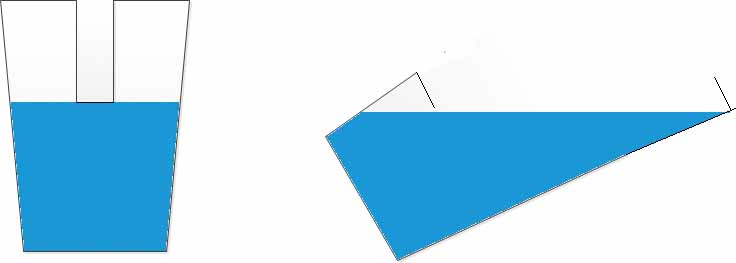
\includegraphics[width=1\linewidth]{7}
	\caption{木桶原理的短板效应与长板效应}
	\label{fig:1}
\end{figure}

在今天,你认为机柜掉电的可能性会很高吗?如果你的答案是肯定的,那么分散到两个机柜后就没有问题了吗?要是按照这种逻辑思考,即便分散到两个机柜,整个数据中心不是也有掉电的可能吗?如此一来,难道你还要将它们分散到不同的数据中心去吗?

解决基础架构的问题,永远都是先从整体入手。如果我们把个体问题排在前面,那你的整体规划永远也实现不了。在小地方徘徊,会陷入一个无底洞。如果业务A要考虑,那么业务B、业务C和业务D呢?这样一弄,自己就把自己给搞死了。

其实,一个机柜里最多不过二三十台设备。与其在细枝末节上浪费精力,还不如把整体的可靠性做扎实来得实在。如果电力系统能提供足够的保障,还有什么可纠结的呢?抓大放小,把关键点落实好,其他问题自然就迎刃而解了。在这一点上,思维模式必须要上升到一个更高的层级。随着体量的增加,所能实施冗余的手段也会越来越丰富。比如使用分布式的设计结构、多机房冗余等。完善整体架构才是消除个体问题最好的手段。

6.成本核算时需要考虑什么

数据中心是一个持续性投入的项目,因此我们必须对采购成本加以控制。既然它是按照机柜数量来付费的,那我们是不是可以这样理解:用最少的机柜,上最多的设备。说白了,就是提升上架率。当然,这不是绝对的。上架率并不是越高越好。如果一个机柜最多能容纳25台服务器,你真的会把它上满吗?我想没有人会这么做,因为根本就没有25口的交换机。

首先要明确设备的能耗值,这个值和服务器的配置有关。然后据此计算最佳的设备上架率,将上架设备的数量调整到一个适合的范围,使之和选用交换机的产品规格相适应。不要一边提升了上架率,另一边又增加了网络资源的开销。

在进行计算成本的时候,会涉及如下几组概念与公式。

(1)机柜有效容量

这项参数直接反映了机柜的容纳能力,它的高低取决于电力容量、空间和设备能耗之间的匹配程度。计算机柜有效容量可以使用公式3-1来完成。

\begin{figure}[htbp]
	\centering
	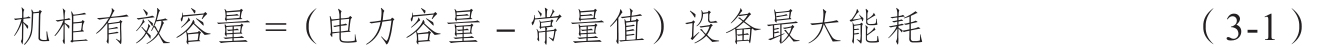
\includegraphics[width=1\linewidth]{8}
	\caption{}
	\label{fig:1}
\end{figure}

公式1中的常量值是指除服务器之外的设备能耗,比如TOR交换机。由于交换机的能耗比较低,一般在几十瓦到一百多瓦之间,所以它不像服务器那样有比较大的波动。我们可以近似地认为,这个数值是恒定的。TOR交换机至少需要两台,分别用于业务和带外管理。此外,由于有Pod的概念,部分机柜需要增加汇聚层的设备。因此,我们建议将常量值的取值范围定义为1.5~2A。

另外,还要特别注意几点。第一,机柜有效容量指的是服务器的数量,并不包含交换机。第二,这个公式无法消除空间限制所带来的影响。如果机架采用标准U位,设备是无法紧密摆放的。第三,使用最大能耗作除数更保险一些。这样做,是为了防止所有设备同时达到峰值而建立的最后一道防线。



\section{3.4 本章小结}

\chapter{网络规划细节对系统运维的影响}
\section{4.1 案例复盘}
\section{4.2 事情为什么弄得一团糟}
\section{4.3 网络空间资源的规划}
\subsection{4.3.1 PoD容量的计算方法}
\subsection{4.3.2 地址空间的规划}
\subsection{4.3.3 VLAN的规划}
\section{4.4 网卡绑定}
\subsection{4.4.1 网卡绑定模式的选择}
\subsection{4.4.2 网卡绑定的实现}
\section{4.5 本章小结}
\chapter{服务器硬件选型}
\section{5.1 如何选择合适的硬件配置}
\subsection{5.1.1 选型的总体原则}
\subsection{5.1.2 选型中值得注意的地方}
\section{5.2 怎样的一款服务器产品才算是优秀的}
\subsection{5.2.1 带外管理有多重要}
\subsection{5.2.2 异构平台融合能力}
\subsection{5.2.3 完善的信息数据展示}
\subsection{5.2.4 软硬件环境兼容性}
\subsection{5.2.5 用户体验}
\section{5.3 产品测试那些事儿}
\subsection{5.3.1 测试前的准备工作}
\subsection{5.3.2 部署系统测试}
\subsection{5.3.3 产品功能性测试}
\subsection{5.3.4 能耗测试}
\subsection{5.3.5 CPU性能测试}
\subsection{5.3.6 内存性能测试}
\subsection{5.3.7 磁盘性能测试}
\subsection{5.3.8 网络性能测试}
\subsection{5.3.9 测试后的收尾工作}
\section{5.4 本章小结}
\chapter{构建CMDB与Workflow}
\section{6.1 谁拖了运维的后腿}
\section{6.2 定海神针CMDB}
\subsection{6.2.1 CMDB是一切运维的基石}
\subsection{6.2.2 是什么毁了CMDB}
\subsection{6.2.3 如何定义你的需求}
\subsection{6.2.4 如何定义表结构}
\subsection{6.2.5 设计思想原则}
\section{6.3 多面娇娃Workflow}
\subsection{6.3.1 一份周报中竟然80%的工作量都是在沟通}
\subsection{6.3.2 Workflow能干什么}
\subsection{6.3.3 Workflow是实例化的规范}
\subsection{6.3.4 Workflow是领航员}
\subsection{6.3.5 Workflow设计中的常见问题}
\section{6.4 本章小结}
\chapter{构建IaaS平台系统}
\section{7.1 高效交付解决方案如何选型}
\section{7.2 服务器设置详解}
\subsection{7.2.1 IPMI}
\subsection{7.2.2 racadmin}
\subsection{7.2.3 SMASH CLP}
\section{7.3 Cobbler部署系统详解}
\subsection{7.3.1 理解Cobbler架构}
\subsection{7.3.2 Cobbler的安装配置}
\subsection{7.3.3 命名规范}
\subsection{7.3.4 创建资源目录}
\subsection{7.3.5 创建Cobbler部署模板与实例}
\subsection{7.3.6 Cobbler里面出现的坑}
\section{7.4 IaaS系统的设计要点}
\subsection{7.4.1 交付工作流程定义}
\subsection{7.4.2 Portal模块与各组件之间的调用关系}
\section{7.5 制作KVM虚拟机模板}
\subsection{7.5.1 虚拟机网络环境部署}
\subsection{7.5.2 创建虚拟机镜像模板}
\subsection{7.5.3 虚拟机克隆}
\subsection{7.5.4 虚拟机设备调整}
\subsection{7.5.5 VPC的支持}
\section{7.6 本章小结}
\chapter{构建域名解析服务}
\section{8.1 写在前面的话}
\section{8.2 首先做好一个传统的DNS管理员}
\section{8.3 Anycast DNS在多数据中心中的应用}
\subsection{8.3.1 什么是Anycast}
\subsection{8.3.2 如何构建DNS over Anycast}
\subsection{8.3.3 如何实施Anycast DNS}
\subsection{8.3.4 如何守护quagga进程}
\subsection{8.3.5 BGP在Anycast中的应用}
\section{8.4 HTTP DNS}
\subsection{8.4.1 传统DNS的缺陷}
\subsection{8.4.2 HTTP DNS的优势}
\subsection{8.4.3 HTTP DNS长什么样}
\subsection{8.4.4 HTTP DNS会取代传统的DNS吗}
\section{8.5 本章小结}
\chapter{时间同步系统}
\section{9.1 概述}
\subsection{9.1.1 如何实现时间同步}
\subsection{9.1.2 GPS卫星系统授时原理}
\subsection{9.1.3 PTP}
\subsection{9.1.4 为何要选用硬件时间源服务器}
\subsection{9.1.5 如何选择硬件时间源服务器}
\section{9.2 ntpd}
\subsection{9.2.1 ntpd初始化}
\subsection{9.2.2 ntpd配置文件}
\subsection{9.2.3 使用ntpq查询时间同步的状态}
\section{9.3 chronyd}
\subsection{9.3.1 chronyd的优势}
\subsection{9.3.2 chronyd配置文件}
\subsection{9.3.3 使用key限制客户端访问}
\subsection{9.3.4 跟踪时间同步过程}
\subsection{9.3.5 检查时间同步状态}
\section{9.4 如何处理闰秒}
\subsection{9.4.1 闰秒是什么}
\subsection{9.4.2 闰秒的危害}
\subsection{9.4.3 前辈们是怎么解决闰秒的}
\subsection{9.4.4 晦涩难懂的术语}
\subsection{9.4.5 怎么解决闰秒问题}
\section{9.5 本章小结}
\chapter{配置管理}
\section{10.1 本章目的}
\section{10.2 expect与Parallel SSH}
\subsection{10.2.1 expect}
\subsection{10.2.2 Parallel SSH}
\subsection{10.2.3 SSH的通病}
\section{10.3 Ansible}
\subsection{10.3.1 创建Host Inventory}
\subsection{10.3.2 如何自动添加节点}
\subsection{10.3.3 组织主机节点}
\subsection{10.3.4 Ad-Hoc}
\subsection{10.3.5 Playbook}
\subsection{10.3.6 关于优化}
\section{10.4 Puppet}
\subsection{10.4.1 Puppet快跑}
\subsection{10.4.2 初探Puppet}
\subsection{10.4.3 使用Apache+Passenger替换WEBRick}
\subsection{10.4.4 Mutil-Master\&Mutil-CAServer}
\subsection{10.4.5 排障}
\section{10.5 SaltStack}
\subsection{10.5.1 配置Minion}
\subsection{10.5.2 管理Salt Key}
\subsection{10.5.3 组织主机节点}
\subsection{10.5.4 模块的调用}
\subsection{10.5.5 Mutil-Masters}
\subsection{10.5.6 级联}
\subsection{10.5.7 SLS}
\subsection{10.5.8 Grain}
\subsection{10.5.9 Pillar}
\subsection{10.5.10 排障}
\section{10.6 我们真的能抗住海量节点吗}
\subsection{10.6.1 集合编队}
\subsection{10.6.2 汇报战况}
\subsection{10.6.3 不必过度依赖模块}
\section{10.7 解决方案的选择}
\section{10.8 本章小结}
\chapter{文件共享服务}
\section{11.1 构建WebDAV服务}
\subsection{11.1.1 基本构建}
\subsection{11.1.2 WebDAV on HTTPS}
\section{11.2 构建NFS服务}
\subsection{11.2.1 NFS v4的新特性}
\subsection{11.2.2 NFS常见问题处理}
\subsection{11.2.3 NFS高可用方案}
\subsection{11.2.4 NFS Cluster实施条件}
\subsection{11.2.5 NFS Cluster的实施}
\subsection{11.2.6 NFS Cluster故障排错}
\section{11.3 构建SFTP服务}
\subsection{11.3.1 Chroot SFTP和公钥访问的必要性}
\subsection{11.3.2 构建Chroot SFTP}
\subsection{11.3.3 SFTP容灾方案}
\section{11.4 本章小结}
\chapter{硬件故障告警与维修}
\section{12.1 硬件故障的特点}
\section{12.2 硬件故障告警}
\subsection{12.2.1 告警方式}
\subsection{12.2.2 事件类型和告警级别}
\section{12.3 硬件故障分析}
\subsection{12.3.1 常用分析手段}
\subsection{12.3.2 常见故障错误分析}
\section{12.4 传统维修的问题}
\section{12.5 报修系统的需求定义}
\subsection{12.5.1 故障申报环节的设计需求}
\subsection{12.5.2 审批通告环节的设计需求}
\subsection{12.5.3 提交报修环节的设计需求}
\subsection{12.5.4 设备维修环节的设计需求}
\subsection{12.5.5 数据查询统计的设计需求}
\section{12.6 本章小结}
\chapter{主机系统信息安全基础}
\section{13.1 系统安全加固的基本要求}
\section{13.2 关于安全配置的反思}
\subsection{13.2.1 慎用账户锁定}
\subsection{13.2.2 密码的烦恼}
\subsection{13.2.3 sudo的意义}
\section{13.3 sudo over LDAP的实现}
\subsection{13.3.1 服务端配置}
\subsection{13.3.2 客户端配置}
\subsection{13.3.3 关于LDAP超时和连接数限制的问题}
\section{13.4 密码学与数字证书}
\subsection{13.4.1 密码学技术}
\subsection{13.4.2 数据加密与数字签名}
\subsection{13.4.3 公钥加密体系的安全性论述}
\subsection{13.4.4 数字证书是什么}
\subsection{13.4.5 数字证书是怎么产生的}
\subsection{13.4.6 数字证书是怎么验证的}
\section{13.5 人为因素}
\subsection{13.5.1 运维红线}
\subsection{13.5.2 安全操作}
\subsection{13.5.3 运维工作中的常见问题}
\section{13.6 本章小结}
\chapter{性能校准}
\section{14.1 队列理论}
\section{14.2 CPU}
\subsection{14.2.1 来自内核态的资源消耗}
\subsection{14.2.2 用户态资源占用率高}
\subsection{14.2.3 Cache与内存的三种映射关系}
\subsection{14.2.4 CPU调度算法}
\subsection{14.2.5 进程运行在哪个核心上}
\subsection{14.2.6 strace的妙用}
\section{14.3 内存}
\subsection{14.3.1 NUMA}
\subsection{14.3.2 Cache和Buffer}
\subsection{14.3.3 虚拟地址空间}
\subsection{14.3.4 大页}
\subsection{14.3.5 内存分配}
\subsection{14.3.6 内存回收}
\subsection{14.3.7 内存超配了怎么办}
\subsection{14.3.8 为什么会产生OOM}
\section{14.4 存储}
\subsection{14.4.1 磁盘调度算法}
\subsection{14.4.2 I/O调度算法}
\subsection{14.4.3 日志模式}
\subsection{14.4.4 其他因素}
\section{14.5 网络}
\subsection{14.5.1 Jumbo Frames}
\subsection{14.5.2 BDP}
\subsection{14.5.3 qperf}
\subsection{14.5.4 其他}
\section{14.6 本章小结}
\chapter{Shell编程}
\section{15.1 参数传递}
\subsection{15.1.1 shift}
\subsection{15.1.2 eval}
\subsection{15.1.3 getopt}
\subsection{15.1.4 函数传参}
\subsection{15.1.5 返回值}
\section{15.2 文本处理三剑客}
\subsection{15.2.1 grep}
\subsection{15.2.2 sed}
\subsection{15.2.3 awk}
\section{15.3 字符处理}
\subsection{15.3.1 字符的转义}
\subsection{15.3.2 字符串截取}
\section{15.4 数组}
\section{15.5 算来算去}
\subsection{15.5.1 比较}
\subsection{15.5.2 字符串计算}
\subsection{15.5.3 精度与长度}
\subsection{15.5.4 进制转换}
\section{15.6 表面文章}
\section{15.7 典型案例}
\section{15.8 本章小结}
\chapter{修行之路}
\section{16.1 系统工程师的自我修养}
\subsection{16.1.1 工程师与管理员}
\subsection{16.1.2 系统工程师的三颗心}
\subsection{16.1.3 匠人精神}
\section{16.2 未来时代}
\subsection{16.2.1 前方高能——出现怪兽AlphaGo}
\subsection{16.2.2 从现在开始就要改变自己}
\subsection{16.2.3 开启你的管理模式}
\section{16.3 写在最后的话}

\backmatter

IT基础架构:系统运维实践
赵旻 著
ISBN:978-7-111-59778-0



\end{document}